% Options for packages loaded elsewhere
% Options for packages loaded elsewhere
\PassOptionsToPackage{unicode}{hyperref}
\PassOptionsToPackage{hyphens}{url}
\PassOptionsToPackage{dvipsnames,svgnames,x11names}{xcolor}
%
\documentclass[
  letterpaper,
  DIV=11,
  numbers=noendperiod]{scrartcl}
\usepackage{xcolor}
\usepackage{amsmath,amssymb}
\setcounter{secnumdepth}{5}
\usepackage{iftex}
\ifPDFTeX
  \usepackage[T1]{fontenc}
  \usepackage[utf8]{inputenc}
  \usepackage{textcomp} % provide euro and other symbols
\else % if luatex or xetex
  \usepackage{unicode-math} % this also loads fontspec
  \defaultfontfeatures{Scale=MatchLowercase}
  \defaultfontfeatures[\rmfamily]{Ligatures=TeX,Scale=1}
\fi
\usepackage{lmodern}
\ifPDFTeX\else
  % xetex/luatex font selection
\fi
% Use upquote if available, for straight quotes in verbatim environments
\IfFileExists{upquote.sty}{\usepackage{upquote}}{}
\IfFileExists{microtype.sty}{% use microtype if available
  \usepackage[]{microtype}
  \UseMicrotypeSet[protrusion]{basicmath} % disable protrusion for tt fonts
}{}
\usepackage{setspace}
% Make \paragraph and \subparagraph free-standing
\makeatletter
\ifx\paragraph\undefined\else
  \let\oldparagraph\paragraph
  \renewcommand{\paragraph}{
    \@ifstar
      \xxxParagraphStar
      \xxxParagraphNoStar
  }
  \newcommand{\xxxParagraphStar}[1]{\oldparagraph*{#1}\mbox{}}
  \newcommand{\xxxParagraphNoStar}[1]{\oldparagraph{#1}\mbox{}}
\fi
\ifx\subparagraph\undefined\else
  \let\oldsubparagraph\subparagraph
  \renewcommand{\subparagraph}{
    \@ifstar
      \xxxSubParagraphStar
      \xxxSubParagraphNoStar
  }
  \newcommand{\xxxSubParagraphStar}[1]{\oldsubparagraph*{#1}\mbox{}}
  \newcommand{\xxxSubParagraphNoStar}[1]{\oldsubparagraph{#1}\mbox{}}
\fi
\makeatother


\usepackage{longtable,booktabs,array}
\usepackage{calc} % for calculating minipage widths
% Correct order of tables after \paragraph or \subparagraph
\usepackage{etoolbox}
\makeatletter
\patchcmd\longtable{\par}{\if@noskipsec\mbox{}\fi\par}{}{}
\makeatother
% Allow footnotes in longtable head/foot
\IfFileExists{footnotehyper.sty}{\usepackage{footnotehyper}}{\usepackage{footnote}}
\makesavenoteenv{longtable}
\usepackage{graphicx}
\makeatletter
\newsavebox\pandoc@box
\newcommand*\pandocbounded[1]{% scales image to fit in text height/width
  \sbox\pandoc@box{#1}%
  \Gscale@div\@tempa{\textheight}{\dimexpr\ht\pandoc@box+\dp\pandoc@box\relax}%
  \Gscale@div\@tempb{\linewidth}{\wd\pandoc@box}%
  \ifdim\@tempb\p@<\@tempa\p@\let\@tempa\@tempb\fi% select the smaller of both
  \ifdim\@tempa\p@<\p@\scalebox{\@tempa}{\usebox\pandoc@box}%
  \else\usebox{\pandoc@box}%
  \fi%
}
% Set default figure placement to htbp
\def\fps@figure{htbp}
\makeatother





\setlength{\emergencystretch}{3em} % prevent overfull lines

\providecommand{\tightlist}{%
  \setlength{\itemsep}{0pt}\setlength{\parskip}{0pt}}



 
\usepackage[round]{natbib}
\bibliographystyle{apalike}


\usepackage{fontspec}
\usepackage{multirow}
\usepackage{multicol}
\usepackage{colortbl}
\usepackage{hhline}
\newlength\Oldarrayrulewidth
\newlength\Oldtabcolsep
\usepackage{longtable}
\usepackage{array}
\usepackage{hyperref}
\usepackage{float}
\usepackage{wrapfig}
% \usepackage{hyperref}
% \hypersetup{
%     colorlinks,
%     linkcolor={blue!100!black},
%     citecolor={blue!100!black},
%     urlcolor={blue!100!black}
% }
% \usepackage{apacite}
% \usepackage[round]{natbib} 
% \usepackage{graphicx}
% \usepackage{float}
% \usepackage{caption}
% \usepackage[toc,page]{appendix}
% \usepackage{booktabs,caption}
% \usepackage[flushleft]{threeparttable}
% \usepackage{tabularx}
\usepackage{sfmath}
\usepackage{fontspec}
\usepackage[utf8]{inputenc}
\usepackage{siunitx}
\usepackage{amsfonts}
\usepackage{amsmath}
% \usepackage{xcolor}
% \usepackage{scrextend}
% \deffootnote[2em]{2em}{1em}{\textsuperscript{\thefootnotemark}\,}
% \newcolumntype{Y}{>{\centering\arraybackslash}X}
% \usepackage[a4paper]{geometry}
% \usepackage{caption}
% \usepackage[bottom,flushmargin,hang,multiple]{footmisc}
% \usepackage{pdflscape}
% \usepackage[paper=portrait,pagesize]{typearea}
% \usepackage{rotating}
% \usepackage{fullpage}
% \usepackage{tabu}
\usepackage{lscape}
\newcommand{\blandscape}{\begin{landscape}}
\newcommand{\elandscape}{\end{landscape}}
\usepackage{rotating}
\newcommand{\bsideways}{\begin{sidewaystable}[htbp]}
\newcommand{\esideways}{\end{sidewaystable}}
\KOMAoption{captions}{tableheading}
\makeatletter
\@ifpackageloaded{caption}{}{\usepackage{caption}}
\AtBeginDocument{%
\ifdefined\contentsname
  \renewcommand*\contentsname{Table of contents}
\else
  \newcommand\contentsname{Table of contents}
\fi
\ifdefined\listfigurename
  \renewcommand*\listfigurename{List of Figures}
\else
  \newcommand\listfigurename{List of Figures}
\fi
\ifdefined\listtablename
  \renewcommand*\listtablename{List of Tables}
\else
  \newcommand\listtablename{List of Tables}
\fi
\ifdefined\figurename
  \renewcommand*\figurename{Figure}
\else
  \newcommand\figurename{Figure}
\fi
\ifdefined\tablename
  \renewcommand*\tablename{Table}
\else
  \newcommand\tablename{Table}
\fi
}
\@ifpackageloaded{float}{}{\usepackage{float}}
\floatstyle{ruled}
\@ifundefined{c@chapter}{\newfloat{codelisting}{h}{lop}}{\newfloat{codelisting}{h}{lop}[chapter]}
\floatname{codelisting}{Listing}
\newcommand*\listoflistings{\listof{codelisting}{List of Listings}}
\makeatother
\makeatletter
\makeatother
\makeatletter
\@ifpackageloaded{caption}{}{\usepackage{caption}}
\@ifpackageloaded{subcaption}{}{\usepackage{subcaption}}
\makeatother
\usepackage{bookmark}
\IfFileExists{xurl.sty}{\usepackage{xurl}}{} % add URL line breaks if available
\urlstyle{same}
\hypersetup{
  colorlinks=true,
  linkcolor={blue!100!black},
  filecolor={Maroon},
  citecolor={blue!100!black},
  urlcolor={blue!100!black},
  pdfcreator={LaTeX via pandoc}}


\author{}
\date{}
\begin{document}

\title{Do investors in clean energy ETFs herd? The role of climate risks}



\author{ 
Vassilios Babalos\footnote{Corresponding Author. Department of Accounting and Finance, University of Peloponnese, Kalamata,  Greece; Email: v.babalos@uop.gr.} \,\,
Xolani Sibande\footnote{Department of Economics, University of Pretoria, Pretoria, South Africa; Email: xolaniss@gmail.com. Economic Research Department, South African Reserve Bank, Pretoria, South Africa.} \,\, 
Elie Bouri\footnote{Adnan Kassar School of Business, Lebanese American University, Lebanon; Email: elie.elbouri@lau.edu.lb} \,\,
Rangan Gupta\footnote{Department of Economics, University of Pretoria, Pretoria, South Africa; Email: rangan.gupta@up.ac.za.} 
}
\date{\today}
\maketitle

\begin{abstract}

\textbf{Purpose} -- This study investigates herding behaviour in US clean energy Exchange-traded funds (ETFs) and examines the role of climate risks in influencing such behaviour over the period from May 1, 2016 to June 19, 2024.

\textbf{Design/methodology/approach} -- We employ a baseline herding model and extend it to examine asymmetric effects across market conditions. The analysis incorporates time-varying herding measures and examines the impact of both transitional and physical climate risks on herding probability using regression techniques.

\textbf{Findings} -- The baseline model reveals significant herding behaviour in clean energy ETFs. The extended model indicates that herding is present in both down and up markets, with a stronger effect in down markets, suggesting asymmetry. Herding is also found to be time-varying. Notably, high levels of transitional climate risk reduce the probability of herding in clean energy ETFs, whereas physical climate risk does not exert any significant impact on herding probability.

\textbf{Research limitations/implications} -- The study focuses specifically on US clean energy ETFs over a defined period, which may limit generalizability to other markets or asset classes. The findings provide insights into the behavioral dynamics of sustainable investment markets during periods of varying climate risk.

\textbf{Practical implications} -- The results suggest that high levels of transitional climate risk encourage market efficiency in clean energy ETFs and promote climate-hedging behaviour by investors. This has important implications for portfolio managers and policymakers in understanding market dynamics in sustainable finance.

\textbf{Originality/value} -- This study provides novel empirical evidence on the relationship between climate risks and herding behaviour in clean energy ETFs, contributing to the growing literature on behavioral finance in sustainable investment markets.

\end{abstract}

\noindent\textbf{Keywords}: Herding Behaviour, Climate Change, Clean Energy
\\
\textbf{JEL Codes}: G14, Q54, P18
\newpage


\setstretch{1.5}
\section{Introduction}\label{introduction}

Climate sustainability is a major concern for financial markets and
investors. The growing interest in climate sustainability is primarily
driven by the increasing materialisation of climate risks, and the
actions of governments, institutions and organizations towards a
sustainable future \citep{giglio2021a}. To safeguard returns, investors
increasingly seek to hedge against climate risks by investing in green
financial products. Although the evidence from the existing literature
is mixed, returns from green financial products are somewhat comparable
to traditional financial products \citetext{\citealp[see amongst
others,][]{decclesia2024}; \citealp{nguyen2025}; \citealp{pastor2022}; \citealp[and][]{naqvi2022}}.
In this new climate sustainability paradigm, investors face many
pressures that not only bear on returns but also the stability of
financial markets. For example, resulting regulations aimed at reducing
emissions can surprisingly reduce the profitability of fossil-fuel-based
companies, or the possible mispricing of assets from ignoring climate
risks can lead to significant losses \citep{nguyen2025}. In addition to
climate risks, a general change in investor attitudes can drive the
inclusion of green assets in their portfolio can lead to systemic
risk.\footnote{These pressures notwithstanding the possible contribution
  that financial markets can play in mitigating and reducing the
  negative effects of climate change \citep{giglio2021a}} Specifically,
climate change presents risks to the global financial system, and
ultimately to investment portfolios, through two primary sources -
physical and transition risks. Physical risks or direct impact refer to
extreme climate events such as floods and droughts, which impact
business operations and infrastructure; and transition risks are the
policy, technological, and other costs that societies bear to achieve
low carbon economies \citetext{\citealp{nguyen2025}; \citealp[and][
amongst others]{giglio2021a}}. Investors, therefore, recognise these
risks and seek to mitigate them, as they seek return-enhancing green
financial products.

Energy market has been in the epicentre of retail investors and
portfolio managers at least over the last two decades. Official
estimates claim that global energy investment is expected to surpass USD
3 trillion for the first time in 2024, with USD 2 trillion going to
clean energy technologies and infrastructure \citep{iea2024}. There is a
general consensus in the literature that the most important event that
has shaped the current landscape in the energy sector is the emergence
of the energy portfolio with the rise of green energy as an alternative
energy resource and an asset class. Price volatility of fossil fuels on
the one hand and decarbonisation-related goals dictated by international
agreements on the other hand are heavily responsible for the growing
interest in green energy market. Responding to the increasing awareness
about the environment and the need for more green capital, financial
markets have also attracted a large portion of retail and institutional
investors' fund flows \citep{rizvi2022green, naqvi2021there}.

Needless to mention that the rise of energy popularity as an alternative
investment class has also been fueled by the fictionalization of
commodities markets. Commodities have become an effective investment
tool for investment community as it allows investors to participate in
the market developments across various physical products such as
agricultural products, silver, gold, natural gas, oil etc and more
recently clean energy products without being obliged to own the product
directly \citep{gagnon2020they}. Several academic studies have
highlighted substantial diversification benefits of commodities when
added to a portfolio of stocks and bonds \citep[see inter
alia,][]{naqvi2022}.

Green energy sectors like solar, wind, geothermal, biofuels, biomass,
wave, hydro and tidal energies are considered by investors, authorities
and policy-makers as the substitutes for fossil-fuels energy that
increase \(CO_2\) emissions \citep{shahzad2020clean}. Moreover, as
\citet{naqvi2022} point out that ``the alternative energy sector is
expected to grow faster over the next decades due to the depletion of
fossil fuel reserves and the technological advance that has made green
energy feasible''.

Although green energy investment has witnessed an exponential growth
over the years, there is a lot of improvement that can be done in terms
of investors' participation, both retail and institutional. To achieve
the goal of larger capital commitment to green energy projects it is
important to gain investors' confidence in financial products that are
linked to green energy such as Exchange-traded funds(ETFs).

ETFs are a key feature of green financial products. They are a
collection of investments that often tracks an underlying performance of
an asset or index. In the universe of environment, social, and
governance (ESG) investments, clean ETFs serve as a tool for
environmentally conscious investors to identify and invest in
environmentally friendly companies \citep{briere2023} engaged in the
transition towards a cleaner production and a low-carbon economy. Among
the ESG ETFs, the Clean Energy (CE) ETFs have been the best-performing
one in 2022 \citep{decclesia2024}. This is not surprising given that the
clean energy transition represents one of the largest multi-decade
secular growth opportunities. After the inclusion of Green energy
financing in the list of United Nations Sustainability Goals (SDGs) as
SDG 7, the role, importance, and visibility of green financial products
have escalated enormously \citep{naqvi2022}. That is, the growth of
green assets under management is likely to continue. Furthermore, the
limited availability of data on ESG complying investment tools
\citep{avramov2022, nguyen2025} justifies the use of energy ETFs as best
candidates of green assets. However, given that the inclusion of climate
sustainability in investment decisions is a recent phenomenon, it is not
clear what the actual impact will be in the long-run.

This study investigates herding behaviour in alternative (clean) energy
ETFs in the US between May 1 2016 and June 19 2024, showing evidence of
significant herding that is asymmetric and time-varying. We then study
whether climate-related uncertainty can affect the herding behaviour in
the US clean energy ETFs market. Methodologically, we follow the
standard herding tests by \citet{christie1995} and \citet{chang2000}.
Notably, we supplement the traditional approach with quantile
regressions \citep{koenker1978} in order to capture how herding differs
across various quantiles of the returns dispersion and in up and down
markets. Lastly, to establish a link between climate risk and herding
behaviour, we differentiating between transitional and physical risks
\citep{bua2024} and provide valuable insights on their potential impact
on the likelihood of herding in clean energy ETFs.

In this study specifically, we ask whether the rapid adoption of clean
energy ETFs could be driven by market fads, or is a fundamental change
in investor behaviour. Investors, for example, can believe that their
peers have more valuable information about climate risks, making them to
herd to avoid losses compared to peers; alternatively, investors may be
encouraged to herd by the desire to align to climate-related social
values \citep{ciciretti2021, gavrilakis2023, loang2023}. Investors in
clean energy stocks can experience large losses if their betting on
clean energy stocks go wrong, which represents a major concern in their
decision-making process. This incites those investors to disregard their
own information and follow the market consensus, leading to significant
herding behaviour in the clean energy market. \citet{devenow1996}
indicate that following the market consensus induces some kind of
security among less informed traders. This could be relevant to our
analysis because ETFs represent a popular investment instrument for
individual and retail investors who are not necessarily well informed
about the risk and prospects of investments in clean energy firms and
whether their contribution to the world transition to cleaner production
should be financially lucrative. On a related front, the
self-reinforcing nature of confidence in the tyranny of the majority, as
indicated by \citet{teraji2003} could also be pertinent.

While herding behaviour has been examined in ESG markets, it remains
understudied in clean energy assets, notably, clean energy
ETFs.\footnote{Amongst others, \citet{loang2023} shows that compliance
  with SDG goals can introduce bias in investor sentiment, which leads
  to herding behaviour. Using a Twitter (or X) uncertainty index,
  \citet{koutmos2024} finds evidence of herding in US-based ESG index
  fund investors. \citet{przychodzen2016} found indicate evidence of
  herding behaviour amongst fund managers who incorporated ESG
  strategies in their portfolios. Lastly, \citet{rubbaniy2021} highlight
  evidence of herding in the MSCI US ESG Leader Index during extreme
  (bear and bull periods) periods.} Other studies on herding have been
conducted in commodity and fossil energy markets. For example,
\citet{demirer2013} conducted a commodity sectoral study and found
herding behaviour in grains but not in other sectors. Similarly,
\citet{gilbert2010} shows herding behaviour amongst speculators in
non-ferrous commodities. Others did not find evidence of herding in
similar markets. \citet{babalos2015} find significant anti-herding
behaviour in metal commodities futures after the global financial
crisis. \citet{pierdzioch2010} show that forecasters in oil and metals
markets deviated from the crowd, indicating a rational response to
market information. \citet{steen2013} find no herding behaviour in
international commodity markets. Notably, our study extends the results
of \citet{dragomirescu-gaina2021} who have examined herding behaviour of
investors in the US energy sector and herding sensitivity to various
proxies of policy uncertainty and financial risk. They study the energy
equities included in the S\&P 500 and concluded that herding among
investors in the US energy market sector is sensitive to green
volatility shocks

Our analysis shows that herding is significant and is present in both
down and up markets, with a stronger effect in the down market,
suggesting an asymmetry. Herding is also found to be time-varying.
Notably, an additional analysis reveals that the transition climate
risk, particularly its high level, reduces the probability of herding in
clean energy ETFs, whereas physical climate risk does not exert any
significant impact on the probability of herding

The next section describes the data and methodology, followed by the
results and conclusions.

\section{Data and methodology}\label{data-and-methodology}

\subsection{Data}\label{data}

The sample consists of clean energy equity ETFs (green ETFs) that are
traded in the US markets (see Table~\ref{tbl-data} in the
Appendix).\footnote{The data were sourced from
  \url{https://datastream.org/en-ca/}} The number of available clean
energy ETFs in our sample varied from 10 in the beginning of analysis to
30 at the most. The period of analysis runs from May 1 2016 to 19 June
2024. Daily closing prices on the clean energy ETFs under study were
collected from the Refinitiv database. The starting date was selected on
the basis of the UN Climate Change Conference (COP) Paris agreement.
Daily logarithmic returns were computed from the closing prices of each
ETF, yielding, a total of 2122 observations per ETF.

\begin{figure}[H]

\centering{

\pandocbounded{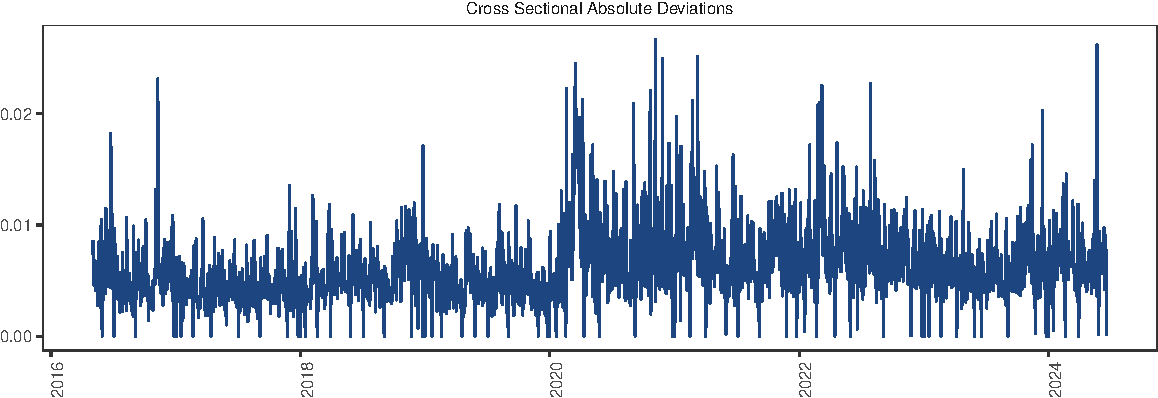
\includegraphics[keepaspectratio]{alt_energy_herding_final_files/figure-pdf/fig-csad-1.pdf}}

}

\caption{\label{fig-csad}Cross Sectional Absolute Deviation (CSAD) for
US Alternative Energy ETFs}

\end{figure}%

The development of the CSAD measure over time for the clean energy ETFs
is presented in Figure~\ref{fig-csad}. In general, the CSAD measure
remains within certain bounds. However, we observe several cases when
the CSAD measure deviates significantly from the market consensus:
around the announcement of the Paris agreement (2016-2017), the covid-19
pandemic crisis (2020--2021), the war outbreak in Ukraine (2022) among
others. Table~\ref{tbl-desc} presents the descriptive statistics of the
data.

\global\setlength{\Oldarrayrulewidth}{\arrayrulewidth}

\global\setlength{\Oldtabcolsep}{\tabcolsep}

\setlength{\tabcolsep}{2pt}

\renewcommand*{\arraystretch}{0.7}



\providecommand{\ascline}[3]{\noalign{\global\arrayrulewidth #1}\arrayrulecolor[HTML]{#2}\cline{#3}}

\begin{longtable}[l]{|p{1.46in}|p{1.08in}|p{1.08in}|p{1.23in}|p{1.14in}}

\caption{\label{tbl-desc}Descriptive statistics of the data}

\tabularnewline

\ascline{1pt}{000000}{1-5}

\multicolumn{1}{!{\color[HTML]{FFFFFF}\vrule width 1pt}>{\raggedright}m{\dimexpr 1.46in+0\tabcolsep}}{\textcolor[HTML]{000000}{\fontsize{7}{7}\selectfont{\global\setmainfont{Arial}{\ }}}} & \multicolumn{1}{!{\color[HTML]{FFFFFF}\vrule width 1pt}>{\centering}m{\dimexpr 1.08in+0\tabcolsep}}{\textcolor[HTML]{000000}{\fontsize{7}{7}\selectfont{\global\setmainfont{Arial}{Mean}}}} & \multicolumn{1}{!{\color[HTML]{FFFFFF}\vrule width 1pt}>{\centering}m{\dimexpr 1.08in+0\tabcolsep}}{\textcolor[HTML]{000000}{\fontsize{7}{7}\selectfont{\global\setmainfont{Arial}{St.dev}}}} & \multicolumn{1}{!{\color[HTML]{FFFFFF}\vrule width 1pt}>{\centering}m{\dimexpr 1.23in+0\tabcolsep}}{\textcolor[HTML]{000000}{\fontsize{7}{7}\selectfont{\global\setmainfont{Arial}{Skewness}}}} & \multicolumn{1}{!{\color[HTML]{FFFFFF}\vrule width 1pt}>{\centering}m{\dimexpr 1.14in+0\tabcolsep}!{\color[HTML]{FFFFFF}\vrule width 1pt}}{\textcolor[HTML]{000000}{\fontsize{7}{7}\selectfont{\global\setmainfont{Arial}{Kurtosis}}}} \\

\ascline{1pt}{000000}{1-5}\endfirsthead 

\ascline{1pt}{000000}{1-5}

\multicolumn{1}{!{\color[HTML]{FFFFFF}\vrule width 1pt}>{\raggedright}m{\dimexpr 1.46in+0\tabcolsep}}{\textcolor[HTML]{000000}{\fontsize{7}{7}\selectfont{\global\setmainfont{Arial}{\ }}}} & \multicolumn{1}{!{\color[HTML]{FFFFFF}\vrule width 1pt}>{\centering}m{\dimexpr 1.08in+0\tabcolsep}}{\textcolor[HTML]{000000}{\fontsize{7}{7}\selectfont{\global\setmainfont{Arial}{Mean}}}} & \multicolumn{1}{!{\color[HTML]{FFFFFF}\vrule width 1pt}>{\centering}m{\dimexpr 1.08in+0\tabcolsep}}{\textcolor[HTML]{000000}{\fontsize{7}{7}\selectfont{\global\setmainfont{Arial}{St.dev}}}} & \multicolumn{1}{!{\color[HTML]{FFFFFF}\vrule width 1pt}>{\centering}m{\dimexpr 1.23in+0\tabcolsep}}{\textcolor[HTML]{000000}{\fontsize{7}{7}\selectfont{\global\setmainfont{Arial}{Skewness}}}} & \multicolumn{1}{!{\color[HTML]{FFFFFF}\vrule width 1pt}>{\centering}m{\dimexpr 1.14in+0\tabcolsep}!{\color[HTML]{FFFFFF}\vrule width 1pt}}{\textcolor[HTML]{000000}{\fontsize{7}{7}\selectfont{\global\setmainfont{Arial}{Kurtosis}}}} \\

\ascline{1pt}{000000}{1-5}\endhead



\multicolumn{1}{!{\color[HTML]{FFFFFF}\vrule width 1pt}>{\raggedright}m{\dimexpr 1.46in+0\tabcolsep}}{\textcolor[HTML]{000000}{\fontsize{7}{7}\selectfont{\global\setmainfont{Arial}{CSAD}}}} & \multicolumn{1}{!{\color[HTML]{FFFFFF}\vrule width 1pt}>{\centering}m{\dimexpr 1.08in+0\tabcolsep}}{\textcolor[HTML]{000000}{\fontsize{7}{7}\selectfont{\global\setmainfont{Arial}{0.0062}}}} & \multicolumn{1}{!{\color[HTML]{FFFFFF}\vrule width 1pt}>{\centering}m{\dimexpr 1.08in+0\tabcolsep}}{\textcolor[HTML]{000000}{\fontsize{7}{7}\selectfont{\global\setmainfont{Arial}{0.0034}}}} & \multicolumn{1}{!{\color[HTML]{FFFFFF}\vrule width 1pt}>{\centering}m{\dimexpr 1.23in+0\tabcolsep}}{\textcolor[HTML]{000000}{\fontsize{7}{7}\selectfont{\global\setmainfont{Arial}{1.5598}}}} & \multicolumn{1}{!{\color[HTML]{FFFFFF}\vrule width 1pt}>{\centering}m{\dimexpr 1.14in+0\tabcolsep}!{\color[HTML]{FFFFFF}\vrule width 1pt}}{\textcolor[HTML]{000000}{\fontsize{7}{7}\selectfont{\global\setmainfont{Arial}{7.9355}}}} \\

\ascline{1pt}{FFFFFF}{1-5}



\multicolumn{1}{!{\color[HTML]{FFFFFF}\vrule width 1pt}>{\raggedright}m{\dimexpr 1.46in+0\tabcolsep}}{\textcolor[HTML]{000000}{\fontsize{7}{7}\selectfont{\global\setmainfont{Arial}{Absolute\ CSAR}}}} & \multicolumn{1}{!{\color[HTML]{FFFFFF}\vrule width 1pt}>{\centering}m{\dimexpr 1.08in+0\tabcolsep}}{\textcolor[HTML]{000000}{\fontsize{7}{7}\selectfont{\global\setmainfont{Arial}{0.0094}}}} & \multicolumn{1}{!{\color[HTML]{FFFFFF}\vrule width 1pt}>{\centering}m{\dimexpr 1.08in+0\tabcolsep}}{\textcolor[HTML]{000000}{\fontsize{7}{7}\selectfont{\global\setmainfont{Arial}{0.0107}}}} & \multicolumn{1}{!{\color[HTML]{FFFFFF}\vrule width 1pt}>{\centering}m{\dimexpr 1.23in+0\tabcolsep}}{\textcolor[HTML]{000000}{\fontsize{7}{7}\selectfont{\global\setmainfont{Arial}{3.3175}}}} & \multicolumn{1}{!{\color[HTML]{FFFFFF}\vrule width 1pt}>{\centering}m{\dimexpr 1.14in+0\tabcolsep}!{\color[HTML]{FFFFFF}\vrule width 1pt}}{\textcolor[HTML]{000000}{\fontsize{7}{7}\selectfont{\global\setmainfont{Arial}{23.8725}}}} \\

\ascline{1pt}{000000}{1-5}


\end{longtable}

\arrayrulecolor[HTML]{000000}

\global\setlength{\arrayrulewidth}{\Oldarrayrulewidth}

\global\setlength{\tabcolsep}{\Oldtabcolsep}

\renewcommand*{\arraystretch}{1}

\subsection{Methodology}\label{methodology}

It is well established that herding literature is vast with
contradictory results depending mainly on the market, the employed
methodology and the period under consideration \citep{spyrou2013}.
Herding behaviour can be either spurious in cases when investors make
similar decisions as a result of processing the same information set and
intentional herding when investors imitate the actions of others
\citep[see inter alia][]{bikhchandani2000, galariotis2015}. Empirical
studies on herding usually fall into two categories: namely those that
employ holdings data aiming at measuring institutional investor herding
\citep[e.g.][]{lakonishok1992}, and studies that use market returns data
and investigate herding towards the market consensus
\citep[e.g.][]{chang2000, galariotis2015}. Our paper falls within the
latter category and tests for herding towards the market consensus for
clean energy US ETFs.

More broadly, studies that focus on herding can be broadly classified
into two main categories: on the one hand there are studies that examine
institutional investor herding and analyst herding using
transaction-level data
\citetext{\citealp{lakonishok1992}; \citealp[and][among
others]{sias2004institutional}}. On the other hand, there are studies
that explore herding towards the market consensus employing individual
returns and market returns
\citetext{\citealp{christie1995}; \citealp[and][]{chang2000}}. In the
latter case, the most widely employed method is the cross-sectional
standard deviation of returns proposed by \citet{christie1995}. The
intuition behind this approach is that herding toward the market is
signaled when return dispersion is relatively low. Rational asset
pricing theory predicts that when stocks respond to market movements in
various degrees then dispersion will be linearly related to market
returns \citep[see also,][]{hwang2004market}. However, when investors
tend to mimic each other and herd towards the market the linear relation
between returns dispersion and aggregate market returns is no longer
valid. Under these conditions, fitting a non-linear regression
specification between a measure of returns dispersion and aggregate
market return appears as a more viable choice. Therefore, our approach
to measure herding activity is based on the non-linear regression model
by \citet{chang2000}.

Following this relevant literature, we compute dispersion of the
\(i^{th}\) ETF from the market return, which is known as the Cross
Sectional Absolute Deviation (\(CSAD_t\)) measure. Empirically the
\(CSAD_t\) is defined in the following manner:

\begin{equation}\phantomsection\label{eq-csad}{
CSAD_t = \dfrac{1}{N}\sum_{i=1}^{N} |R_{i,t} - R_{m,t}|,
}\end{equation}

where \(R_{i,t}\) is the return and \(R_{m,t}\) is the cross sectional
average of returns for the sample of ETFs available for each day. The
return dispersion measures the directional similarity of ETF returns to
the market return. This return similarity forms the basis for the
herding behaviour tests. Following \citet{galariotis2015} we estimate
Equation~\ref{eq-herding}:

\begin{equation}\phantomsection\label{eq-herding}{
CSAD_t = \gamma_0 + \gamma_1 |R_{m,t}| + \gamma_2 R_{m,t}^2 + \epsilon_t,
}\end{equation}

where \(\gamma_0\) is the intercept, \(\gamma_1\) is the coefficient of
the linear term, \(\gamma_2\) is the coefficient of the quadratic term
or the herding behaviour term, and \(\epsilon_t\) is the error term. The
coefficient \(\gamma_2 <0\) when herding is present, and \(\gamma_2 >0\)
when anti-herding is present. To ensure the robustness of the estimate,
we estimate \(CSAD_{t}\) with Newey-West standard errors
\citep[See][]{newey1987}.

To provide additional insight on the herding phenomenon we examine
whether herding presents an asymmetric response on days when the market
is up vis-à-vis days when the market is down. To this end, we augment
Equation~\ref{eq-herding} as follows:

\begin{equation}\phantomsection\label{eq-asymmetry}{
CSAD_t = \gamma_0 + \gamma_1(1-D) R_{m,t} + \gamma_2D R_{m,t} + \gamma_3(1-D) R_{m,t}^2  + \gamma_4D R_{m,t}^2 + \epsilon_t,
}\end{equation}

where \(D\) is a dummy variable that takes the value of 1 when the
market return is negative and 0 otherwise. Therefore, our exploration of
asymmetric behaviour of herding phenomenon is carried through the
inspection of the statistical significance and the sign of the two
estimated coefficients \(\gamma_3\) versus \(\gamma_4\) (up versus down
markets).

\section{Results}\label{results}

\subsection{Herding behaviour}\label{herding-behaviour}

Rational asset pricing models \citep[for example,][]{black1972} predict
a linear relationship between return dispersion and market returns under
normal conditions, a relationship that is no longer valid in the
presence of herding. Herding behaviour leads to an increasing or
decreasing cross sectional dispersion with respect to market returns. In
other words, herding is captured by a non-linear term in the standard
pricing equation indicating a decreasing or an increasing returns'
dispersion. Stated differently, as \citet{chang2000} argue, in the case
of herding the coefficient on the non-linear term (\(\gamma_2\)) will be
negative and statistically significant.

Table~\ref{tbl-herding} presents the results of herding for the full
sample, based on Equation~\ref{eq-herding}. The estimated coefficient on
market return is positive and highly significant as expected.
Importantly, the estimated coefficient on the non-linear term is
negative (-1.2773) and statistically significant with a t-statistic of
-9.71 suggesting that herd behaviour is present and robust in the US
alternative energy ETFs. Accordingly, investors in US clean energy ETFs
tend to disregard their private information and follow market consensus.

\global\setlength{\Oldarrayrulewidth}{\arrayrulewidth}

\global\setlength{\Oldtabcolsep}{\tabcolsep}

\setlength{\tabcolsep}{2pt}

\renewcommand*{\arraystretch}{0.9}



\providecommand{\ascline}[3]{\noalign{\global\arrayrulewidth #1}\arrayrulecolor[HTML]{#2}\cline{#3}}

\begin{longtable}[l]{|p{1.99in}|p{1.99in}|p{1.99in}}

\caption{\label{tbl-herding}Estimation results of herding in the U.S.
equity alternative energy ETFs}

\tabularnewline

\ascline{1pt}{000000}{1-3}

\multicolumn{1}{!{\color[HTML]{FFFFFF}\vrule width 1pt}>{\centering}m{\dimexpr 1.99in+0\tabcolsep}}{\textcolor[HTML]{000000}{\fontsize{7}{7}\selectfont{\global\setmainfont{Arial}{$\gamma_0$}}}} & \multicolumn{1}{!{\color[HTML]{FFFFFF}\vrule width 1pt}>{\centering}m{\dimexpr 1.99in+0\tabcolsep}}{\textcolor[HTML]{000000}{\fontsize{7}{7}\selectfont{\global\setmainfont{Arial}{$\gamma_1 $}}}} & \multicolumn{1}{!{\color[HTML]{FFFFFF}\vrule width 1pt}>{\centering}m{\dimexpr 1.99in+0\tabcolsep}!{\color[HTML]{FFFFFF}\vrule width 1pt}}{\textcolor[HTML]{000000}{\fontsize{7}{7}\selectfont{\global\setmainfont{Arial}{$\gamma_2$}}}} \\

\ascline{1pt}{000000}{1-3}\endfirsthead 

\ascline{1pt}{000000}{1-3}

\multicolumn{1}{!{\color[HTML]{FFFFFF}\vrule width 1pt}>{\centering}m{\dimexpr 1.99in+0\tabcolsep}}{\textcolor[HTML]{000000}{\fontsize{7}{7}\selectfont{\global\setmainfont{Arial}{$\gamma_0$}}}} & \multicolumn{1}{!{\color[HTML]{FFFFFF}\vrule width 1pt}>{\centering}m{\dimexpr 1.99in+0\tabcolsep}}{\textcolor[HTML]{000000}{\fontsize{7}{7}\selectfont{\global\setmainfont{Arial}{$\gamma_1 $}}}} & \multicolumn{1}{!{\color[HTML]{FFFFFF}\vrule width 1pt}>{\centering}m{\dimexpr 1.99in+0\tabcolsep}!{\color[HTML]{FFFFFF}\vrule width 1pt}}{\textcolor[HTML]{000000}{\fontsize{7}{7}\selectfont{\global\setmainfont{Arial}{$\gamma_2$}}}} \\

\ascline{1pt}{000000}{1-3}\endhead



\multicolumn{1}{!{\color[HTML]{FFFFFF}\vrule width 1pt}>{\centering}m{\dimexpr 1.99in+0\tabcolsep}}{\textcolor[HTML]{000000}{\fontsize{7}{7}\selectfont{\global\setmainfont{Arial}{0.0038**}}}} & \multicolumn{1}{!{\color[HTML]{FFFFFF}\vrule width 1pt}>{\centering}m{\dimexpr 1.99in+0\tabcolsep}}{\textcolor[HTML]{000000}{\fontsize{7}{7}\selectfont{\global\setmainfont{Arial}{0.2883***}}}} & \multicolumn{1}{!{\color[HTML]{FFFFFF}\vrule width 1pt}>{\centering}m{\dimexpr 1.99in+0\tabcolsep}!{\color[HTML]{FFFFFF}\vrule width 1pt}}{\textcolor[HTML]{000000}{\fontsize{7}{7}\selectfont{\global\setmainfont{Arial}{\ -1.2773***}}}} \\

\ascline{1pt}{FFFFFF}{1-3}



\multicolumn{1}{!{\color[HTML]{FFFFFF}\vrule width 1pt}>{\centering}m{\dimexpr 1.99in+0\tabcolsep}}{\textcolor[HTML]{000000}{\fontsize{7}{7}\selectfont{\global\setmainfont{Arial}{(47.09)}}}} & \multicolumn{1}{!{\color[HTML]{FFFFFF}\vrule width 1pt}>{\centering}m{\dimexpr 1.99in+0\tabcolsep}}{\textcolor[HTML]{000000}{\fontsize{7}{7}\selectfont{\global\setmainfont{Arial}{(33.333)}}}} & \multicolumn{1}{!{\color[HTML]{FFFFFF}\vrule width 1pt}>{\centering}m{\dimexpr 1.99in+0\tabcolsep}!{\color[HTML]{FFFFFF}\vrule width 1pt}}{\textcolor[HTML]{000000}{\fontsize{7}{7}\selectfont{\global\setmainfont{Arial}{(-9.71)}}}} \\

\ascline{1pt}{000000}{1-3}



\multicolumn{3}{>{\raggedright}m{\dimexpr 5.96in+4\tabcolsep}}{\textcolor[HTML]{000000}{\fontsize{7}{7}\selectfont{\global\setmainfont{Arial}{Note:\ *,**,***\ denotes\ significance\ at\ 10\%,5\%\ and\ 1\%\ respectively.}}}} \\

\ascline{1pt}{000000}{1-3}


\end{longtable}

\arrayrulecolor[HTML]{000000}

\global\setlength{\arrayrulewidth}{\Oldarrayrulewidth}

\global\setlength{\tabcolsep}{\Oldtabcolsep}

\renewcommand*{\arraystretch}{1}

Evidence from the existing literature shows that herding behaviour in
various asset markets \citep[see][]{pochea2017} exhibits asymmetry. To
this end, we proceed first with the estimation of
Equation~\ref{eq-herding} using the quantile regression (QR) proposed by
\citet{koenker1978}. Table~\ref{tbl-quantile_herding} presents the
estimated results across various quantiles of the returns dispersion.
They show that herding is statistically significant at lower
(\(\tau= 25\%\)), middle (\(\tau =50\%\)), and upper (\(\tau=75\%\))
with a value of -1.1056, -1.165, and -1.1473, respectively. No
significant herding is found at extreme lower quantile (\(\tau=10\%\))
and extreme higher quantile (\(\tau=90\%\)).

\global\setlength{\Oldarrayrulewidth}{\arrayrulewidth}

\global\setlength{\Oldtabcolsep}{\tabcolsep}

\setlength{\tabcolsep}{2pt}

\renewcommand*{\arraystretch}{0.7}



\providecommand{\ascline}[3]{\noalign{\global\arrayrulewidth #1}\arrayrulecolor[HTML]{#2}\cline{#3}}

\begin{longtable}[l]{|p{1.49in}|p{1.49in}|p{1.49in}|p{1.49in}}

\caption{\label{tbl-quantile_herding}Estimation results of herding
across various quantiles}

\tabularnewline

\ascline{1pt}{000000}{1-4}

\multicolumn{1}{!{\color[HTML]{FFFFFF}\vrule width 1pt}>{\centering}m{\dimexpr 1.49in+0\tabcolsep}}{\textcolor[HTML]{000000}{\fontsize{7}{7}\selectfont{\global\setmainfont{Arial}{Quantile}}}} & \multicolumn{1}{!{\color[HTML]{FFFFFF}\vrule width 1pt}>{\centering}m{\dimexpr 1.49in+0\tabcolsep}}{\textcolor[HTML]{000000}{\fontsize{7}{7}\selectfont{\global\setmainfont{Arial}{$\gamma_0$}}}} & \multicolumn{1}{!{\color[HTML]{FFFFFF}\vrule width 1pt}>{\centering}m{\dimexpr 1.49in+0\tabcolsep}}{\textcolor[HTML]{000000}{\fontsize{7}{7}\selectfont{\global\setmainfont{Arial}{$\gamma_1 $}}}} & \multicolumn{1}{!{\color[HTML]{FFFFFF}\vrule width 1pt}>{\centering}m{\dimexpr 1.49in+0\tabcolsep}!{\color[HTML]{FFFFFF}\vrule width 1pt}}{\textcolor[HTML]{000000}{\fontsize{7}{7}\selectfont{\global\setmainfont{Arial}{$\gamma_2$}}}} \\

\ascline{1pt}{000000}{1-4}\endfirsthead 

\ascline{1pt}{000000}{1-4}

\multicolumn{1}{!{\color[HTML]{FFFFFF}\vrule width 1pt}>{\centering}m{\dimexpr 1.49in+0\tabcolsep}}{\textcolor[HTML]{000000}{\fontsize{7}{7}\selectfont{\global\setmainfont{Arial}{Quantile}}}} & \multicolumn{1}{!{\color[HTML]{FFFFFF}\vrule width 1pt}>{\centering}m{\dimexpr 1.49in+0\tabcolsep}}{\textcolor[HTML]{000000}{\fontsize{7}{7}\selectfont{\global\setmainfont{Arial}{$\gamma_0$}}}} & \multicolumn{1}{!{\color[HTML]{FFFFFF}\vrule width 1pt}>{\centering}m{\dimexpr 1.49in+0\tabcolsep}}{\textcolor[HTML]{000000}{\fontsize{7}{7}\selectfont{\global\setmainfont{Arial}{$\gamma_1 $}}}} & \multicolumn{1}{!{\color[HTML]{FFFFFF}\vrule width 1pt}>{\centering}m{\dimexpr 1.49in+0\tabcolsep}!{\color[HTML]{FFFFFF}\vrule width 1pt}}{\textcolor[HTML]{000000}{\fontsize{7}{7}\selectfont{\global\setmainfont{Arial}{$\gamma_2$}}}} \\

\ascline{1pt}{000000}{1-4}\endhead



\multicolumn{1}{!{\color[HTML]{FFFFFF}\vrule width 1pt}>{\centering}m{\dimexpr 1.49in+0\tabcolsep}}{\textcolor[HTML]{000000}{\fontsize{7}{7}\selectfont{\global\setmainfont{Arial}{$\tau = 10\%$}}}} & \multicolumn{1}{!{\color[HTML]{FFFFFF}\vrule width 1pt}>{\centering}m{\dimexpr 1.49in+0\tabcolsep}}{\textcolor[HTML]{000000}{\fontsize{7}{7}\selectfont{\global\setmainfont{Arial}{0.0016***}}}} & \multicolumn{1}{!{\color[HTML]{FFFFFF}\vrule width 1pt}>{\centering}m{\dimexpr 1.49in+0\tabcolsep}}{\textcolor[HTML]{000000}{\fontsize{7}{7}\selectfont{\global\setmainfont{Arial}{0.2536***}}}} & \multicolumn{1}{!{\color[HTML]{FFFFFF}\vrule width 1pt}>{\centering}m{\dimexpr 1.49in+0\tabcolsep}!{\color[HTML]{FFFFFF}\vrule width 1pt}}{\textcolor[HTML]{000000}{\fontsize{7}{7}\selectfont{\global\setmainfont{Arial}{\ -1.3736}}}} \\

\ascline{1pt}{FFFFFF}{1-4}



\multicolumn{1}{!{\color[HTML]{FFFFFF}\vrule width 1pt}>{\centering}m{\dimexpr 1.49in+0\tabcolsep}}{\textcolor[HTML]{000000}{\fontsize{7}{7}\selectfont{\global\setmainfont{Arial}{$\tau = 25\%$}}}} & \multicolumn{1}{!{\color[HTML]{FFFFFF}\vrule width 1pt}>{\centering}m{\dimexpr 1.49in+0\tabcolsep}}{\textcolor[HTML]{000000}{\fontsize{7}{7}\selectfont{\global\setmainfont{Arial}{0.0026***}}}} & \multicolumn{1}{!{\color[HTML]{FFFFFF}\vrule width 1pt}>{\centering}m{\dimexpr 1.49in+0\tabcolsep}}{\textcolor[HTML]{000000}{\fontsize{7}{7}\selectfont{\global\setmainfont{Arial}{0.2461***}}}} & \multicolumn{1}{!{\color[HTML]{FFFFFF}\vrule width 1pt}>{\centering}m{\dimexpr 1.49in+0\tabcolsep}!{\color[HTML]{FFFFFF}\vrule width 1pt}}{\textcolor[HTML]{000000}{\fontsize{7}{7}\selectfont{\global\setmainfont{Arial}{\ -1.1056***}}}} \\

\ascline{1pt}{FFFFFF}{1-4}



\multicolumn{1}{!{\color[HTML]{FFFFFF}\vrule width 1pt}>{\centering}m{\dimexpr 1.49in+0\tabcolsep}}{\textcolor[HTML]{000000}{\fontsize{7}{7}\selectfont{\global\setmainfont{Arial}{$\tau = 50\%$}}}} & \multicolumn{1}{!{\color[HTML]{FFFFFF}\vrule width 1pt}>{\centering}m{\dimexpr 1.49in+0\tabcolsep}}{\textcolor[HTML]{000000}{\fontsize{7}{7}\selectfont{\global\setmainfont{Arial}{0.0037***}}}} & \multicolumn{1}{!{\color[HTML]{FFFFFF}\vrule width 1pt}>{\centering}m{\dimexpr 1.49in+0\tabcolsep}}{\textcolor[HTML]{000000}{\fontsize{7}{7}\selectfont{\global\setmainfont{Arial}{0.2648***}}}} & \multicolumn{1}{!{\color[HTML]{FFFFFF}\vrule width 1pt}>{\centering}m{\dimexpr 1.49in+0\tabcolsep}!{\color[HTML]{FFFFFF}\vrule width 1pt}}{\textcolor[HTML]{000000}{\fontsize{7}{7}\selectfont{\global\setmainfont{Arial}{\ -1.165***}}}} \\

\ascline{1pt}{FFFFFF}{1-4}



\multicolumn{1}{!{\color[HTML]{FFFFFF}\vrule width 1pt}>{\centering}m{\dimexpr 1.49in+0\tabcolsep}}{\textcolor[HTML]{000000}{\fontsize{7}{7}\selectfont{\global\setmainfont{Arial}{$\tau = 75\%$}}}} & \multicolumn{1}{!{\color[HTML]{FFFFFF}\vrule width 1pt}>{\centering}m{\dimexpr 1.49in+0\tabcolsep}}{\textcolor[HTML]{000000}{\fontsize{7}{7}\selectfont{\global\setmainfont{Arial}{0.0048***}}}} & \multicolumn{1}{!{\color[HTML]{FFFFFF}\vrule width 1pt}>{\centering}m{\dimexpr 1.49in+0\tabcolsep}}{\textcolor[HTML]{000000}{\fontsize{7}{7}\selectfont{\global\setmainfont{Arial}{0.3011***}}}} & \multicolumn{1}{!{\color[HTML]{FFFFFF}\vrule width 1pt}>{\centering}m{\dimexpr 1.49in+0\tabcolsep}!{\color[HTML]{FFFFFF}\vrule width 1pt}}{\textcolor[HTML]{000000}{\fontsize{7}{7}\selectfont{\global\setmainfont{Arial}{\ -1.1473***}}}} \\

\ascline{1pt}{FFFFFF}{1-4}



\multicolumn{1}{!{\color[HTML]{FFFFFF}\vrule width 1pt}>{\centering}m{\dimexpr 1.49in+0\tabcolsep}}{\textcolor[HTML]{000000}{\fontsize{7}{7}\selectfont{\global\setmainfont{Arial}{$\tau = 90\%$}}}} & \multicolumn{1}{!{\color[HTML]{FFFFFF}\vrule width 1pt}>{\centering}m{\dimexpr 1.49in+0\tabcolsep}}{\textcolor[HTML]{000000}{\fontsize{7}{7}\selectfont{\global\setmainfont{Arial}{0.0064***}}}} & \multicolumn{1}{!{\color[HTML]{FFFFFF}\vrule width 1pt}>{\centering}m{\dimexpr 1.49in+0\tabcolsep}}{\textcolor[HTML]{000000}{\fontsize{7}{7}\selectfont{\global\setmainfont{Arial}{0.2999***}}}} & \multicolumn{1}{!{\color[HTML]{FFFFFF}\vrule width 1pt}>{\centering}m{\dimexpr 1.49in+0\tabcolsep}!{\color[HTML]{FFFFFF}\vrule width 1pt}}{\textcolor[HTML]{000000}{\fontsize{7}{7}\selectfont{\global\setmainfont{Arial}{\ 0.2314}}}} \\

\ascline{1pt}{000000}{1-4}



\multicolumn{4}{>{\raggedright}m{\dimexpr 5.94in+6\tabcolsep}}{\textcolor[HTML]{000000}{\fontsize{7}{7}\selectfont{\global\setmainfont{Arial}{Note:\ This\ table\ presents\ the\ estimation\ results\ of\ herding\ of\ US\ Alternative\ energy\ equity\ ETFs\ according\ to\ Equation\ 2\ in\ various\ quantiles\ 10,\ 25,\ 50,\ 75\ and\ 90\%\ of\ the\ returns\ distribution.}}}\textcolor[HTML]{000000}{\fontsize{7}{7}\selectfont{\global\setmainfont{Arial}{\ }}}\textcolor[HTML]{000000}{\fontsize{7}{7}\selectfont{\global\setmainfont{Arial}{*,**,***\ denotes\ significance\ at\ 10\%,5\%\ and\ 1\%\ respectively.}}}} \\

\ascline{1pt}{000000}{1-4}


\end{longtable}

\arrayrulecolor[HTML]{000000}

\global\setlength{\arrayrulewidth}{\Oldarrayrulewidth}

\global\setlength{\tabcolsep}{\Oldtabcolsep}

\renewcommand*{\arraystretch}{1}

\subsection{Herding behaviour during extreme market
periods}\label{herding-behaviour-during-extreme-market-periods}

Then, we study herding in up and down markets. It is widely accepted
that asset returns are characterized by asymmetry, that is, return
dispersion tend to behave differently in rising and falling markets
\citep[see][]{geert2000, zhou2013, longin2001}, with evidence suggesting
that herding is more pronounced during periods of market stress. In this
regard, examining the relationship between returns dispersion and
market-wide returns across various quantiles of the returns distribution
of clean energy ETFs allows us to make more robust inference regarding
the true behaviour of the herding phenomenon.
Table~\ref{tbl-asymmetry_herding} reports the estimation results of
herding in the up and down markets based on Equation~\ref{eq-asymmetry}.
In general, we find that herding is significant in both down and up
markets

\newpage

\global\setlength{\Oldarrayrulewidth}{\arrayrulewidth}

\global\setlength{\Oldtabcolsep}{\tabcolsep}

\setlength{\tabcolsep}{2pt}

\renewcommand*{\arraystretch}{0.7}



\providecommand{\ascline}[3]{\noalign{\global\arrayrulewidth #1}\arrayrulecolor[HTML]{#2}\cline{#3}}

\begin{longtable}[l]{|p{0.99in}|p{0.99in}|p{0.99in}|p{0.99in}|p{0.99in}|p{0.99in}}

\caption{\label{tbl-asymmetry_herding}Estimation results of herding in
up and down markets}

\tabularnewline

\ascline{1pt}{000000}{1-6}

\multicolumn{1}{!{\color[HTML]{FFFFFF}\vrule width 1pt}>{\centering}m{\dimexpr 0.99in+0\tabcolsep}}{\textcolor[HTML]{000000}{\fontsize{7}{7}\selectfont{\global\setmainfont{Arial}{Quantile}}}} & \multicolumn{1}{!{\color[HTML]{FFFFFF}\vrule width 1pt}>{\centering}m{\dimexpr 0.99in+0\tabcolsep}}{\textcolor[HTML]{000000}{\fontsize{7}{7}\selectfont{\global\setmainfont{Arial}{$\gamma_0$}}}} & \multicolumn{1}{!{\color[HTML]{FFFFFF}\vrule width 1pt}>{\centering}m{\dimexpr 0.99in+0\tabcolsep}}{\textcolor[HTML]{000000}{\fontsize{7}{7}\selectfont{\global\setmainfont{Arial}{$\gamma_1 $}}}} & \multicolumn{1}{!{\color[HTML]{FFFFFF}\vrule width 1pt}>{\centering}m{\dimexpr 0.99in+0\tabcolsep}}{\textcolor[HTML]{000000}{\fontsize{7}{7}\selectfont{\global\setmainfont{Arial}{$\gamma_2$}}}} & \multicolumn{1}{!{\color[HTML]{FFFFFF}\vrule width 1pt}>{\centering}m{\dimexpr 0.99in+0\tabcolsep}}{\textcolor[HTML]{000000}{\fontsize{7}{7}\selectfont{\global\setmainfont{Arial}{$\gamma_3$}}}} & \multicolumn{1}{!{\color[HTML]{FFFFFF}\vrule width 1pt}>{\centering}m{\dimexpr 0.99in+0\tabcolsep}!{\color[HTML]{FFFFFF}\vrule width 1pt}}{\textcolor[HTML]{000000}{\fontsize{7}{7}\selectfont{\global\setmainfont{Arial}{$\gamma_4$}}}} \\

\ascline{1pt}{000000}{1-6}\endfirsthead 

\ascline{1pt}{000000}{1-6}

\multicolumn{1}{!{\color[HTML]{FFFFFF}\vrule width 1pt}>{\centering}m{\dimexpr 0.99in+0\tabcolsep}}{\textcolor[HTML]{000000}{\fontsize{7}{7}\selectfont{\global\setmainfont{Arial}{Quantile}}}} & \multicolumn{1}{!{\color[HTML]{FFFFFF}\vrule width 1pt}>{\centering}m{\dimexpr 0.99in+0\tabcolsep}}{\textcolor[HTML]{000000}{\fontsize{7}{7}\selectfont{\global\setmainfont{Arial}{$\gamma_0$}}}} & \multicolumn{1}{!{\color[HTML]{FFFFFF}\vrule width 1pt}>{\centering}m{\dimexpr 0.99in+0\tabcolsep}}{\textcolor[HTML]{000000}{\fontsize{7}{7}\selectfont{\global\setmainfont{Arial}{$\gamma_1 $}}}} & \multicolumn{1}{!{\color[HTML]{FFFFFF}\vrule width 1pt}>{\centering}m{\dimexpr 0.99in+0\tabcolsep}}{\textcolor[HTML]{000000}{\fontsize{7}{7}\selectfont{\global\setmainfont{Arial}{$\gamma_2$}}}} & \multicolumn{1}{!{\color[HTML]{FFFFFF}\vrule width 1pt}>{\centering}m{\dimexpr 0.99in+0\tabcolsep}}{\textcolor[HTML]{000000}{\fontsize{7}{7}\selectfont{\global\setmainfont{Arial}{$\gamma_3$}}}} & \multicolumn{1}{!{\color[HTML]{FFFFFF}\vrule width 1pt}>{\centering}m{\dimexpr 0.99in+0\tabcolsep}!{\color[HTML]{FFFFFF}\vrule width 1pt}}{\textcolor[HTML]{000000}{\fontsize{7}{7}\selectfont{\global\setmainfont{Arial}{$\gamma_4$}}}} \\

\ascline{1pt}{000000}{1-6}\endhead



\multicolumn{1}{!{\color[HTML]{FFFFFF}\vrule width 1pt}>{\centering}m{\dimexpr 0.99in+0\tabcolsep}}{\textcolor[HTML]{000000}{\fontsize{7}{7}\selectfont{\global\setmainfont{Arial}{$\tau = 10\%$}}}} & \multicolumn{1}{!{\color[HTML]{FFFFFF}\vrule width 1pt}>{\centering}m{\dimexpr 0.99in+0\tabcolsep}}{\textcolor[HTML]{000000}{\fontsize{7}{7}\selectfont{\global\setmainfont{Arial}{0.0016***}}}} & \multicolumn{1}{!{\color[HTML]{FFFFFF}\vrule width 1pt}>{\centering}m{\dimexpr 0.99in+0\tabcolsep}}{\textcolor[HTML]{000000}{\fontsize{7}{7}\selectfont{\global\setmainfont{Arial}{0.2532***}}}} & \multicolumn{1}{!{\color[HTML]{FFFFFF}\vrule width 1pt}>{\centering}m{\dimexpr 0.99in+0\tabcolsep}}{\textcolor[HTML]{000000}{\fontsize{7}{7}\selectfont{\global\setmainfont{Arial}{\ -1.3669***}}}} & \multicolumn{1}{!{\color[HTML]{FFFFFF}\vrule width 1pt}>{\centering}m{\dimexpr 0.99in+0\tabcolsep}}{\textcolor[HTML]{000000}{\fontsize{7}{7}\selectfont{\global\setmainfont{Arial}{\ -0.2522***}}}} & \multicolumn{1}{!{\color[HTML]{FFFFFF}\vrule width 1pt}>{\centering}m{\dimexpr 0.99in+0\tabcolsep}!{\color[HTML]{FFFFFF}\vrule width 1pt}}{\textcolor[HTML]{000000}{\fontsize{7}{7}\selectfont{\global\setmainfont{Arial}{\ -1.1522}}}} \\

\ascline{1pt}{FFFFFF}{1-6}



\multicolumn{1}{!{\color[HTML]{FFFFFF}\vrule width 1pt}>{\centering}m{\dimexpr 0.99in+0\tabcolsep}}{\textcolor[HTML]{000000}{\fontsize{7}{7}\selectfont{\global\setmainfont{Arial}{$\tau = 25\%$}}}} & \multicolumn{1}{!{\color[HTML]{FFFFFF}\vrule width 1pt}>{\centering}m{\dimexpr 0.99in+0\tabcolsep}}{\textcolor[HTML]{000000}{\fontsize{7}{7}\selectfont{\global\setmainfont{Arial}{0.0026***}}}} & \multicolumn{1}{!{\color[HTML]{FFFFFF}\vrule width 1pt}>{\centering}m{\dimexpr 0.99in+0\tabcolsep}}{\textcolor[HTML]{000000}{\fontsize{7}{7}\selectfont{\global\setmainfont{Arial}{0.2475***}}}} & \multicolumn{1}{!{\color[HTML]{FFFFFF}\vrule width 1pt}>{\centering}m{\dimexpr 0.99in+0\tabcolsep}}{\textcolor[HTML]{000000}{\fontsize{7}{7}\selectfont{\global\setmainfont{Arial}{\ -1.2383**}}}} & \multicolumn{1}{!{\color[HTML]{FFFFFF}\vrule width 1pt}>{\centering}m{\dimexpr 0.99in+0\tabcolsep}}{\textcolor[HTML]{000000}{\fontsize{7}{7}\selectfont{\global\setmainfont{Arial}{\ -0.2477***}}}} & \multicolumn{1}{!{\color[HTML]{FFFFFF}\vrule width 1pt}>{\centering}m{\dimexpr 0.99in+0\tabcolsep}!{\color[HTML]{FFFFFF}\vrule width 1pt}}{\textcolor[HTML]{000000}{\fontsize{7}{7}\selectfont{\global\setmainfont{Arial}{\ -1.1171***}}}} \\

\ascline{1pt}{FFFFFF}{1-6}



\multicolumn{1}{!{\color[HTML]{FFFFFF}\vrule width 1pt}>{\centering}m{\dimexpr 0.99in+0\tabcolsep}}{\textcolor[HTML]{000000}{\fontsize{7}{7}\selectfont{\global\setmainfont{Arial}{$\tau = 50\%$}}}} & \multicolumn{1}{!{\color[HTML]{FFFFFF}\vrule width 1pt}>{\centering}m{\dimexpr 0.99in+0\tabcolsep}}{\textcolor[HTML]{000000}{\fontsize{7}{7}\selectfont{\global\setmainfont{Arial}{0.0038***}}}} & \multicolumn{1}{!{\color[HTML]{FFFFFF}\vrule width 1pt}>{\centering}m{\dimexpr 0.99in+0\tabcolsep}}{\textcolor[HTML]{000000}{\fontsize{7}{7}\selectfont{\global\setmainfont{Arial}{0.2247***}}}} & \multicolumn{1}{!{\color[HTML]{FFFFFF}\vrule width 1pt}>{\centering}m{\dimexpr 0.99in+0\tabcolsep}}{\textcolor[HTML]{000000}{\fontsize{7}{7}\selectfont{\global\setmainfont{Arial}{\ 0.3838}}}} & \multicolumn{1}{!{\color[HTML]{FFFFFF}\vrule width 1pt}>{\centering}m{\dimexpr 0.99in+0\tabcolsep}}{\textcolor[HTML]{000000}{\fontsize{7}{7}\selectfont{\global\setmainfont{Arial}{\ -0.2634***}}}} & \multicolumn{1}{!{\color[HTML]{FFFFFF}\vrule width 1pt}>{\centering}m{\dimexpr 0.99in+0\tabcolsep}!{\color[HTML]{FFFFFF}\vrule width 1pt}}{\textcolor[HTML]{000000}{\fontsize{7}{7}\selectfont{\global\setmainfont{Arial}{\ -1.3144***}}}} \\

\ascline{1pt}{FFFFFF}{1-6}



\multicolumn{1}{!{\color[HTML]{FFFFFF}\vrule width 1pt}>{\centering}m{\dimexpr 0.99in+0\tabcolsep}}{\textcolor[HTML]{000000}{\fontsize{7}{7}\selectfont{\global\setmainfont{Arial}{$\tau = 75\%$}}}} & \multicolumn{1}{!{\color[HTML]{FFFFFF}\vrule width 1pt}>{\centering}m{\dimexpr 0.99in+0\tabcolsep}}{\textcolor[HTML]{000000}{\fontsize{7}{7}\selectfont{\global\setmainfont{Arial}{0.0050***}}}} & \multicolumn{1}{!{\color[HTML]{FFFFFF}\vrule width 1pt}>{\centering}m{\dimexpr 0.99in+0\tabcolsep}}{\textcolor[HTML]{000000}{\fontsize{7}{7}\selectfont{\global\setmainfont{Arial}{0.2500***}}}} & \multicolumn{1}{!{\color[HTML]{FFFFFF}\vrule width 1pt}>{\centering}m{\dimexpr 0.99in+0\tabcolsep}}{\textcolor[HTML]{000000}{\fontsize{7}{7}\selectfont{\global\setmainfont{Arial}{\ 1.3135}}}} & \multicolumn{1}{!{\color[HTML]{FFFFFF}\vrule width 1pt}>{\centering}m{\dimexpr 0.99in+0\tabcolsep}}{\textcolor[HTML]{000000}{\fontsize{7}{7}\selectfont{\global\setmainfont{Arial}{\ -0.2785***}}}} & \multicolumn{1}{!{\color[HTML]{FFFFFF}\vrule width 1pt}>{\centering}m{\dimexpr 0.99in+0\tabcolsep}!{\color[HTML]{FFFFFF}\vrule width 1pt}}{\textcolor[HTML]{000000}{\fontsize{7}{7}\selectfont{\global\setmainfont{Arial}{\ -0.9721***}}}} \\

\ascline{1pt}{FFFFFF}{1-6}



\multicolumn{1}{!{\color[HTML]{FFFFFF}\vrule width 1pt}>{\centering}m{\dimexpr 0.99in+0\tabcolsep}}{\textcolor[HTML]{000000}{\fontsize{7}{7}\selectfont{\global\setmainfont{Arial}{$\tau = 90\%$}}}} & \multicolumn{1}{!{\color[HTML]{FFFFFF}\vrule width 1pt}>{\centering}m{\dimexpr 0.99in+0\tabcolsep}}{\textcolor[HTML]{000000}{\fontsize{7}{7}\selectfont{\global\setmainfont{Arial}{0.0065***}}}} & \multicolumn{1}{!{\color[HTML]{FFFFFF}\vrule width 1pt}>{\centering}m{\dimexpr 0.99in+0\tabcolsep}}{\textcolor[HTML]{000000}{\fontsize{7}{7}\selectfont{\global\setmainfont{Arial}{0.2788***}}}} & \multicolumn{1}{!{\color[HTML]{FFFFFF}\vrule width 1pt}>{\centering}m{\dimexpr 0.99in+0\tabcolsep}}{\textcolor[HTML]{000000}{\fontsize{7}{7}\selectfont{\global\setmainfont{Arial}{\ 1.0169}}}} & \multicolumn{1}{!{\color[HTML]{FFFFFF}\vrule width 1pt}>{\centering}m{\dimexpr 0.99in+0\tabcolsep}}{\textcolor[HTML]{000000}{\fontsize{7}{7}\selectfont{\global\setmainfont{Arial}{\ -0.2942***}}}} & \multicolumn{1}{!{\color[HTML]{FFFFFF}\vrule width 1pt}>{\centering}m{\dimexpr 0.99in+0\tabcolsep}!{\color[HTML]{FFFFFF}\vrule width 1pt}}{\textcolor[HTML]{000000}{\fontsize{7}{7}\selectfont{\global\setmainfont{Arial}{\ -1.2003***}}}} \\

\ascline{1pt}{000000}{1-6}



\multicolumn{6}{>{\raggedright}m{\dimexpr 5.91in+10\tabcolsep}}{\textcolor[HTML]{000000}{\fontsize{7}{7}\selectfont{\global\setmainfont{Arial}{Note:\ This\ table\ presents\ the\ estimation\ results\ of\ herding\ of\ US\ Alternative\ energy\ equity\ ETFs\ according\ to\ Equation\ (3).\ }}}\textcolor[HTML]{000000}{\fontsize{7}{7}\selectfont{\global\setmainfont{Arial}{$\gamma_3$}}}\textcolor[HTML]{000000}{\fontsize{7}{7}\selectfont{\global\setmainfont{Arial}{\ captures\ potential\ herding\ in\ the\ up\ market,\ whereas\ }}}\textcolor[HTML]{000000}{\fontsize{7}{7}\selectfont{\global\setmainfont{Arial}{$\gamma_4$}}}\textcolor[HTML]{000000}{\fontsize{7}{7}\selectfont{\global\setmainfont{Arial}{\ captures\ potential\ herding\ in\ the\ down\ market.\ *,**,***denotes\ significance\ at\ 10\%,5\%\ and\ 1\%\ respectively.}}}} \\

\ascline{1pt}{000000}{1-6}


\end{longtable}

\arrayrulecolor[HTML]{000000}

\global\setlength{\arrayrulewidth}{\Oldarrayrulewidth}

\global\setlength{\tabcolsep}{\Oldtabcolsep}

\renewcommand*{\arraystretch}{1}

When the market is rising, herding is present at all quantiles with a
statistically significant coefficient \(\gamma_3\) ranging from -0.2522
(\(\tau=10\%\)) to -0.2942 (\(\tau=90\%\)) . Similarly, when markets are
declining, investors neglect their own information set and imitate the
actions of others resulting in a highly significant coefficient of
herding (\(\gamma_4\)) across four out of five quantiles, ranging from
-0.9721 to -1,3144. Notably, the coefficient of herding in down market
is larger than in up market, reflecting an asymmetric herding behaviour.

\subsection{Time-varying herding
behaviour}\label{time-varying-herding-behaviour}

There is ample evidence that herding varies with time
\citep[see][]{babalos2015, klein2013, stavroyiannis2019} and intensifies
during crisis periods. In order to gain insights on the time-varying
nature of herding in clean energy ETFs, we conduct a rolling window
analysis. The size of the rolling window is related to the time-scales
of the system (response times), and the aim of the research
\citep{babalos2015}. There is no golden rule for the right size of the
rolling window, there is a trade-off between having a long enough window
to estimate the metrics, and short enough to have a sufficient number of
windows in order to be able to derive a trend. Accordingly, we conduct a
rolling window analysis of 50 observations, and plot in
Figure~\ref{fig-rolling_window} the time evolution of the value of the
estimated significance of the herding coefficient (\(\gamma_2\)).

\begin{figure}[H]

\centering{

\pandocbounded{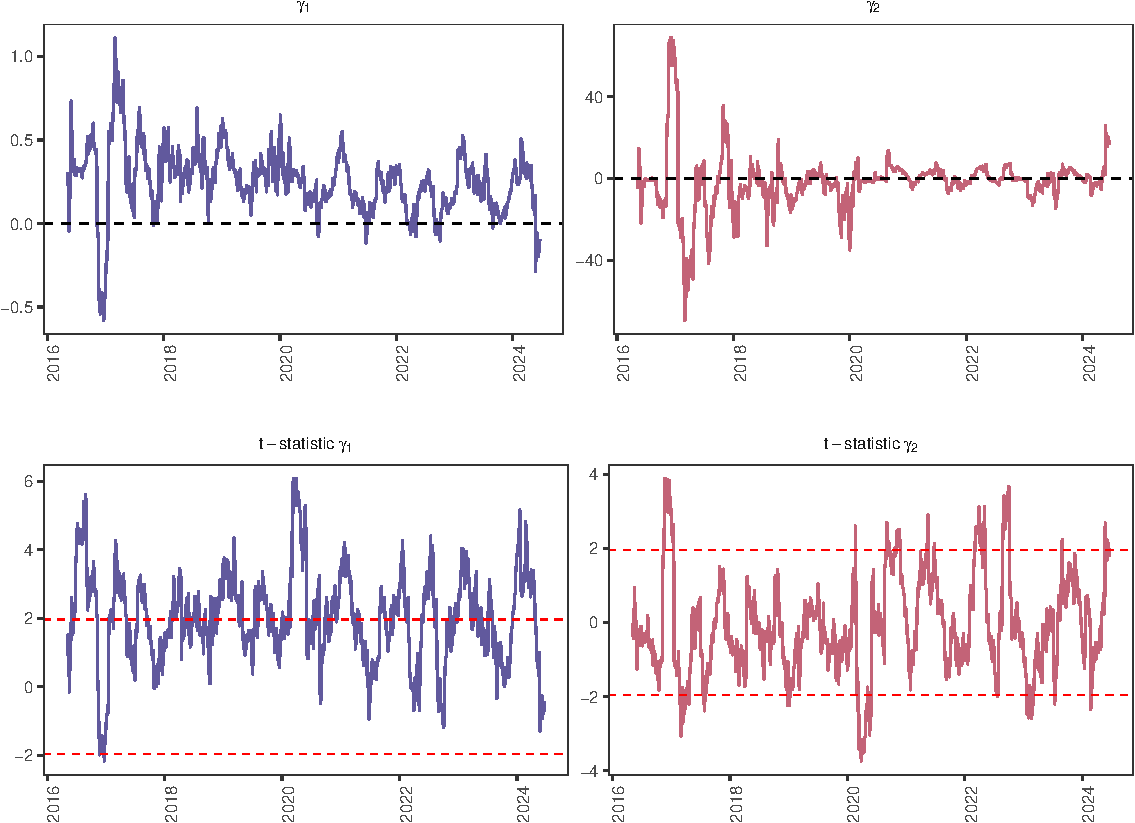
\includegraphics[keepaspectratio]{alt_energy_herding_final_files/figure-pdf/fig-rolling_window-1.pdf}}

}

\caption{\label{fig-rolling_window}Rolling window herding estimates.
Note: The red perforated lines indicates the 95\% confidence interval.}

\end{figure}%

\newpage

We observe several periods of herding behaviour as reflected in the
troughs in Figure~\ref{fig-rolling_window}. The most prominent cases of
herding occur between March and May of 2020 followed by several
instances of herding in the period that extends from March through April
of 2017 and the period of February-March of 2023. On the other side, we
derive significant moments of anti-herding behaviour in the clean energy
ETFs by observing the peaks in Figure~\ref{fig-rolling_window}. Cross
sectional dispersion appears to increase with respect to market-wide
returns, which is a sign of anti-herding behaviour on behalf of
investors around December of 2016 and later during September of 2022

\subsection{Climate risks and herding
behaviour}\label{climate-risks-and-herding-behaviour}

The behaviour of participants in energy markets is closely related to
the developments in the field of climate risks, carbon emissions, and
environmentally friendly policies. Rising climate risk is found to
increase green energy prices \citep{dutta2023}, and evidence from the
existing literature shows that climate policy uncertainty affects the
performance of clean energy stocks relative to dirty ones, making the
former outperform the later when the levels of climate policy
uncertainty are high \citep{bouri2022}. In particular, following the
implementation of the Paris agreement in November 2016, climate policy
uncertainty has become in the epicenter of interest across carbon and
energy markets. There are a few studies that attempt to quantify the
effects of uncertainty related to climate on the economy or financial
markets \citep[see inter alia,][]{gabriel2024, bolton2021, krueger2020}.
Interestingly, \citet{bua2024} developed two climate risk related
indexes namely transition and physical risk using a text-based approach
in order to study the effect of these risks in financial markets. In
this regard, \citet{bouri2023} study the impact of both physical and
climate risks on the returns and volatility of brown and green energy
stocks, carbon emission allowances, and green bonds, showing evidence
that transitional climate risk exerts a more significant impact than
physical climate risk.

It is expected that environmentally conscious investors would prefer to
hold clean energy assets that perform well in the face of increasing
climate change risks \citep[see][]{bouri2022}, even if this entails
accepting lower returns for such climate-hedging assets. Therefore, in
the context of our study and following previous studies on the
determinants of herding behaviour \citep[see][]{bouri2019, demirer2018},
we examine the effect of physical and transition climate risks on the
formation of herding behaviour in the clean energy ETF market.

Furthermore, higher transition risk means greater uncertainty for future
pathway towards a cleaner economy. Under these conditions, green assets
such as green stocks or ETFs are expected to perform better and can
serve as hedging tools \citep[see inter alia][]{pastor}. As a result,
investors allocate their capital to available green assets thus
resulting in higher returns' dispersion with respect to the aggregate
market. Stated differently, investors move their capital away from
market consensus across green ETFs ruling out the possibility of herding
behaviour.

To this end, we use a probit model to relate herding to the two climate
risk indexes developed by \citet{bua2024} in the following manner:

\begin{equation}\phantomsection\label{eq-climate}{
Pr(D^{herd} = 1 |\lambda_0 +  \lambda_1TRI  + \lambda_2PRI) = \lambda_0 +  \lambda_1TRI  + \lambda_2PRI,
}\end{equation}

where \(D^{herd}\) takes a value of 1 during periods of statistically
significant herding (i.e., for days when the rolling t-statistic on
\(\gamma_2 < −1.96\) in Figure~\ref{fig-rolling_window}) and zero
otherwise. \(TRI\) is the transitional risk index and \(PRI\) is the
physical risk index. For details on the construction of \(TRI\) and
\(PRI\), the reader can refer to the paper of \citet{bua2024}.

The results from the Probit model are reported in
Table~\ref{tbl-probit_analysis}. Showing that only the transitional
climate risk index significantly decreases the probability of herding in
clean energy ETFs.\footnote{It should be noted that due to the
  availability of climate risk data from \citet{bua2024}, the probit
  analysis covers the period from May 1, 2016 to December 30, 2023.}
Transitional climate risk represent good news for investors in clean
energy stocks, possibly reducing their self-reinforcing nature of
confidence in the tyranny of the majority \citep{teraji2003} and their
need for shared intention and action, resulting in a decrease in the
herding behaviour. In the presence of higher transitional risk with
respect to the climate, clean energy ETFs become a more attractive
investment alternative for environmentally conscious investors who
allocate their money to alternative energy investment products
\citep[see][]{bouri2022}, reinforcing the confidence of investors in
their own information. As a result, the cross-sectional dispersion of
clean energy ETFs tends to increase. Our results are somewhat in line
with \citet{bouri2023} who show that the transitional climate risk is
more important than physical risk for the return and volatility of clean
energy stocks. They also concord with other relevant studies which
indicate that in the event of climate policy shocks, clean energy assets
could serve the role of hedging instruments \citep{gabriel2024} and tend
to outperform brown energy assets \citep{bouri2022}.

\global\setlength{\Oldarrayrulewidth}{\arrayrulewidth}

\global\setlength{\Oldtabcolsep}{\tabcolsep}

\setlength{\tabcolsep}{2pt}

\renewcommand*{\arraystretch}{0.7}



\providecommand{\ascline}[3]{\noalign{\global\arrayrulewidth #1}\arrayrulecolor[HTML]{#2}\cline{#3}}

\begin{longtable}[l]{|p{3.68in}|p{2.04in}}

\caption{\label{tbl-probit_analysis}Estimation results of the probit
model}

\tabularnewline

\ascline{1pt}{000000}{1-2}

\multicolumn{1}{!{\color[HTML]{FFFFFF}\vrule width 1pt}>{\raggedright}m{\dimexpr 3.68in+0\tabcolsep}}{\textcolor[HTML]{000000}{\fontsize{7}{7}\selectfont{\global\setmainfont{Arial}{Variable}}}} & \multicolumn{1}{!{\color[HTML]{FFFFFF}\vrule width 1pt}>{\centering}m{\dimexpr 2.04in+0\tabcolsep}!{\color[HTML]{FFFFFF}\vrule width 1pt}}{\textcolor[HTML]{000000}{\fontsize{7}{7}\selectfont{\global\setmainfont{Arial}{Coefficient}}}} \\

\ascline{1pt}{000000}{1-2}\endfirsthead 

\ascline{1pt}{000000}{1-2}

\multicolumn{1}{!{\color[HTML]{FFFFFF}\vrule width 1pt}>{\raggedright}m{\dimexpr 3.68in+0\tabcolsep}}{\textcolor[HTML]{000000}{\fontsize{7}{7}\selectfont{\global\setmainfont{Arial}{Variable}}}} & \multicolumn{1}{!{\color[HTML]{FFFFFF}\vrule width 1pt}>{\centering}m{\dimexpr 2.04in+0\tabcolsep}!{\color[HTML]{FFFFFF}\vrule width 1pt}}{\textcolor[HTML]{000000}{\fontsize{7}{7}\selectfont{\global\setmainfont{Arial}{Coefficient}}}} \\

\ascline{1pt}{000000}{1-2}\endhead



\multicolumn{1}{!{\color[HTML]{FFFFFF}\vrule width 1pt}>{\raggedright}m{\dimexpr 3.68in+0\tabcolsep}}{\textcolor[HTML]{000000}{\fontsize{7}{7}\selectfont{\global\setmainfont{Arial}{$\lambda_0$}}}} & \multicolumn{1}{!{\color[HTML]{FFFFFF}\vrule width 1pt}>{\centering}m{\dimexpr 2.04in+0\tabcolsep}!{\color[HTML]{FFFFFF}\vrule width 1pt}}{\textcolor[HTML]{000000}{\fontsize{7}{7}\selectfont{\global\setmainfont{Arial}{\ -1.506***}}}} \\

\ascline{1pt}{FFFFFF}{1-2}



\multicolumn{1}{!{\color[HTML]{FFFFFF}\vrule width 1pt}>{\raggedright}m{\dimexpr 3.68in+0\tabcolsep}}{\textcolor[HTML]{000000}{\fontsize{7}{7}\selectfont{\global\setmainfont{Arial}{$\lambda_1$}}}} & \multicolumn{1}{!{\color[HTML]{FFFFFF}\vrule width 1pt}>{\centering}m{\dimexpr 2.04in+0\tabcolsep}!{\color[HTML]{FFFFFF}\vrule width 1pt}}{\textcolor[HTML]{000000}{\fontsize{7}{7}\selectfont{\global\setmainfont{Arial}{-4.607***}}}} \\

\ascline{1pt}{FFFFFF}{1-2}



\multicolumn{1}{!{\color[HTML]{FFFFFF}\vrule width 1pt}>{\raggedright}m{\dimexpr 3.68in+0\tabcolsep}}{\textcolor[HTML]{000000}{\fontsize{7}{7}\selectfont{\global\setmainfont{Arial}{$\lambda_2$}}}} & \multicolumn{1}{!{\color[HTML]{FFFFFF}\vrule width 1pt}>{\centering}m{\dimexpr 2.04in+0\tabcolsep}!{\color[HTML]{FFFFFF}\vrule width 1pt}}{\textcolor[HTML]{000000}{\fontsize{7}{7}\selectfont{\global\setmainfont{Arial}{-1.318}}}} \\

\ascline{1pt}{000000}{1-2}



\multicolumn{1}{!{\color[HTML]{FFFFFF}\vrule width 1pt}>{\raggedright}m{\dimexpr 3.68in+0\tabcolsep}}{\textcolor[HTML]{000000}{\fontsize{7}{7}\selectfont{\global\setmainfont{Arial}{Log\ Likelihood}}}} & \multicolumn{1}{!{\color[HTML]{FFFFFF}\vrule width 1pt}>{\centering}m{\dimexpr 2.04in+0\tabcolsep}!{\color[HTML]{FFFFFF}\vrule width 1pt}}{\textcolor[HTML]{000000}{\fontsize{7}{7}\selectfont{\global\setmainfont{Arial}{-484.7}}}} \\

\ascline{1pt}{FFFFFF}{1-2}



\multicolumn{1}{!{\color[HTML]{FFFFFF}\vrule width 1pt}>{\raggedright}m{\dimexpr 3.68in+0\tabcolsep}}{\textcolor[HTML]{000000}{\fontsize{7}{7}\selectfont{\global\setmainfont{Arial}{Observations\ with\ Dependent\ Variable\ (Dep)\ =\ 0}}}} & \multicolumn{1}{!{\color[HTML]{FFFFFF}\vrule width 1pt}>{\centering}m{\dimexpr 2.04in+0\tabcolsep}!{\color[HTML]{FFFFFF}\vrule width 1pt}}{\textcolor[HTML]{000000}{\fontsize{7}{7}\selectfont{\global\setmainfont{Arial}{1816}}}} \\

\ascline{1pt}{FFFFFF}{1-2}



\multicolumn{1}{!{\color[HTML]{FFFFFF}\vrule width 1pt}>{\raggedright}m{\dimexpr 3.68in+0\tabcolsep}}{\textcolor[HTML]{000000}{\fontsize{7}{7}\selectfont{\global\setmainfont{Arial}{Observations\ with\ Dependent\ Variable\ (Dep)\ =\ 1}}}} & \multicolumn{1}{!{\color[HTML]{FFFFFF}\vrule width 1pt}>{\centering}m{\dimexpr 2.04in+0\tabcolsep}!{\color[HTML]{FFFFFF}\vrule width 1pt}}{\textcolor[HTML]{000000}{\fontsize{7}{7}\selectfont{\global\setmainfont{Arial}{134}}}} \\

\ascline{1pt}{000000}{1-2}



\multicolumn{2}{>{\raggedright}m{\dimexpr 5.72in+2\tabcolsep}}{\textcolor[HTML]{000000}{\fontsize{7}{7}\selectfont{\global\setmainfont{Arial}{Notes:\ **,***\ denotes\ statistically\ significant\ at\ 5\%\ and\ 1\%}}}} \\

\ascline{1pt}{000000}{1-2}


\end{longtable}

\arrayrulecolor[HTML]{000000}

\global\setlength{\arrayrulewidth}{\Oldarrayrulewidth}

\global\setlength{\tabcolsep}{\Oldtabcolsep}

\renewcommand*{\arraystretch}{1}

Furthermore, we develop two additional models to study the effect of
high and low levels of climate risks on herding behaviour in clean
energy ETFs. Accordingly, we split the sample into two groups based on
the median value of the \(TRI\) and \(PRI\) and estimate the following
two models:

\begin{equation}\phantomsection\label{eq-climate_high}{
Pr(D^{herd} = 1 |\lambda_0 +\lambda_1D^{TRI}_{high}TRI + \lambda_2D^{PRI}_{high}PRI) = \lambda_0 +\lambda_1D^{TRI}_{high}TRI + \lambda_2D^{PRI}_{high}PRI, and
}\end{equation}

\begin{equation}\phantomsection\label{eq-climate_low}{
Pr(D^{herd} = 1 |\lambda_0 +\lambda_1D^{TRI}_{low}TRI + \lambda_2D^{PRI}_{low}PRI) = \lambda_0 +\lambda_1D^{TRI}_{low}TRI + \lambda_2D^{PRI}_{low}PRI, 
}\end{equation}

where \(D^{herd}\) is the same as in Equation~\ref{eq-climate}.
\(D^{TRI}_{high}\) and \(D^{PRI}_{high}\) are dummy variables that take
a value of 1 if the values of the \(TRI\) and \(PRI\) are above the
median and zero otherwise. Similarly, \(D^{TRI}_{low}\) and
\(D^{PRI}_{low}\) are dummy variables that take a value of 1 if the
values of the \(TRI\) and \(PRI\) are below the median and zero
otherwise.

\global\setlength{\Oldarrayrulewidth}{\arrayrulewidth}

\global\setlength{\Oldtabcolsep}{\tabcolsep}

\setlength{\tabcolsep}{2pt}

\renewcommand*{\arraystretch}{0.7}



\providecommand{\ascline}[3]{\noalign{\global\arrayrulewidth #1}\arrayrulecolor[HTML]{#2}\cline{#3}}

\begin{longtable}[l]{|p{2.59in}|p{1.90in}|p{1.86in}}

\caption{\label{tbl-probit_analysis2}Estimation results of the probit
model with high and low climate risk indexes (above or below median)}

\tabularnewline

\ascline{1pt}{000000}{1-3}

\multicolumn{1}{!{\color[HTML]{FFFFFF}\vrule width 1pt}>{\raggedright}m{\dimexpr 2.59in+0\tabcolsep}}{\textcolor[HTML]{000000}{\fontsize{7}{7}\selectfont{\global\setmainfont{Arial}{\ }}}} & \multicolumn{1}{!{\color[HTML]{FFFFFF}\vrule width 1pt}>{\centering}m{\dimexpr 1.9in+0\tabcolsep}}{\textcolor[HTML]{000000}{\fontsize{7}{7}\selectfont{\global\setmainfont{Arial}{High}}}} & \multicolumn{1}{!{\color[HTML]{FFFFFF}\vrule width 1pt}>{\centering}m{\dimexpr 1.86in+0\tabcolsep}!{\color[HTML]{FFFFFF}\vrule width 1pt}}{\textcolor[HTML]{000000}{\fontsize{7}{7}\selectfont{\global\setmainfont{Arial}{Low}}}} \\

\ascline{1pt}{000000}{1-3}\endfirsthead 

\ascline{1pt}{000000}{1-3}

\multicolumn{1}{!{\color[HTML]{FFFFFF}\vrule width 1pt}>{\raggedright}m{\dimexpr 2.59in+0\tabcolsep}}{\textcolor[HTML]{000000}{\fontsize{7}{7}\selectfont{\global\setmainfont{Arial}{\ }}}} & \multicolumn{1}{!{\color[HTML]{FFFFFF}\vrule width 1pt}>{\centering}m{\dimexpr 1.9in+0\tabcolsep}}{\textcolor[HTML]{000000}{\fontsize{7}{7}\selectfont{\global\setmainfont{Arial}{High}}}} & \multicolumn{1}{!{\color[HTML]{FFFFFF}\vrule width 1pt}>{\centering}m{\dimexpr 1.86in+0\tabcolsep}!{\color[HTML]{FFFFFF}\vrule width 1pt}}{\textcolor[HTML]{000000}{\fontsize{7}{7}\selectfont{\global\setmainfont{Arial}{Low}}}} \\

\ascline{1pt}{000000}{1-3}\endhead



\multicolumn{1}{!{\color[HTML]{FFFFFF}\vrule width 1pt}>{\raggedright}m{\dimexpr 2.59in+0\tabcolsep}}{\textcolor[HTML]{000000}{\fontsize{7}{7}\selectfont{\global\setmainfont{Arial}{$\lambda_1$}}}} & \multicolumn{1}{!{\color[HTML]{FFFFFF}\vrule width 1pt}>{\centering}m{\dimexpr 1.9in+0\tabcolsep}}{\textcolor[HTML]{000000}{\fontsize{7}{7}\selectfont{\global\setmainfont{Arial}{-6.736*}}}} & \multicolumn{1}{!{\color[HTML]{FFFFFF}\vrule width 1pt}>{\centering}m{\dimexpr 1.86in+0\tabcolsep}!{\color[HTML]{FFFFFF}\vrule width 1pt}}{\textcolor[HTML]{000000}{\fontsize{7}{7}\selectfont{\global\setmainfont{Arial}{-6.118}}}} \\

\ascline{1pt}{FFFFFF}{1-3}



\multicolumn{1}{!{\color[HTML]{FFFFFF}\vrule width 1pt}>{\raggedright}m{\dimexpr 2.59in+0\tabcolsep}}{\textcolor[HTML]{000000}{\fontsize{7}{7}\selectfont{\global\setmainfont{Arial}{$\lambda_2$}}}} & \multicolumn{1}{!{\color[HTML]{FFFFFF}\vrule width 1pt}>{\centering}m{\dimexpr 1.9in+0\tabcolsep}}{\textcolor[HTML]{000000}{\fontsize{7}{7}\selectfont{\global\setmainfont{Arial}{-1.798}}}} & \multicolumn{1}{!{\color[HTML]{FFFFFF}\vrule width 1pt}>{\centering}m{\dimexpr 1.86in+0\tabcolsep}!{\color[HTML]{FFFFFF}\vrule width 1pt}}{\textcolor[HTML]{000000}{\fontsize{7}{7}\selectfont{\global\setmainfont{Arial}{-2.581}}}} \\

\ascline{1pt}{000000}{1-3}



\multicolumn{3}{>{\raggedright}m{\dimexpr 6.34in+4\tabcolsep}}{\textcolor[HTML]{000000}{\fontsize{7}{7}\selectfont{\global\setmainfont{Arial}{Notes:\ *,\ denotes\ statistically\ significant\ at\ 10\%}}}} \\

\ascline{1pt}{000000}{1-3}


\end{longtable}

\arrayrulecolor[HTML]{000000}

\global\setlength{\arrayrulewidth}{\Oldarrayrulewidth}

\global\setlength{\tabcolsep}{\Oldtabcolsep}

\renewcommand*{\arraystretch}{1}

Using these high \(PRI\) and high \(TRI\) in one probit regression and
low \(TRI\) and low \(PRI\) in another one, we present the results in
Table~\ref{tbl-probit_analysis2}. We observe that high levels of
transition risk decrease the likelihood of herding (i.e.~drives
anti-herding) at the 10\% level of significance, which is in line with
the logic we discussed earlier.

\section{Conclusion}\label{conclusion}

This study offers novel and valuable insights into herding behaviour in
US clean energy ETFs. We used various herding behaviour tests to achieve
this. First, herding is found to be significant, and exists in both
bearish and bullish markets, but shows an asymmetry in that it is more
pronounced in the bearish market. Herding is also found to time-varying.
Second, the transition climate risk, particularly its high levels,
reduce the probability of herding behaviour, whereas physical climate
risk plays no significant role irrespective of its (high or low) levels.
This evidence that climate risks do not lead to higher herding behaviour
in the clean energy ETFs, is new to the related literature.

Our findings offer an interesting outlook on the role of transitional
climate risk for the formation of herding in clean energy ETFs, which is
a puzzle in the related literature. Given that herding represents a
behavioural pattern that can challenge market efficiency and exacerbate
price fluctuations, both policymakers and investors should benefit from
our findings for the sake of investment decision and market efficiency
under the transition towards cleaner production and decarbonized
portfolio investments. Future studies could examine whether herding in
clean energy ETFs is linked to excess volatility in the overall US stock
market.

\newpage

\section*{References}\label{references}
\addcontentsline{toc}{section}{References}

\renewcommand{\bibsection}{}
\bibliography{references.bib}

\setcounter{section}{0}
\renewcommand{\thesection}{\Alph{section}}

\setcounter{table}{0}
\renewcommand{\thetable}{A\arabic{table}}

\setcounter{figure}{0}
\renewcommand{\thefigure}{A\arabic{figure}}

\newpage

\section{Appendix}\label{appendix}

\subsection{ETFs used in the study}\label{etfs-used-in-the-study}

\global\setlength{\Oldarrayrulewidth}{\arrayrulewidth}

\global\setlength{\Oldtabcolsep}{\tabcolsep}

\setlength{\tabcolsep}{2pt}

\renewcommand*{\arraystretch}{0.7}



\providecommand{\ascline}[3]{\noalign{\global\arrayrulewidth #1}\arrayrulecolor[HTML]{#2}\cline{#3}}

\begin{longtable}[l]{|p{5.39in}}

\caption{\label{tbl-data}List of clean energy ETFs used in the study}

\tabularnewline

\ascline{1pt}{000000}{1-1}

\multicolumn{1}{!{\color[HTML]{FFFFFF}\vrule width 1pt}>{\raggedright}m{\dimexpr 5.39in+0\tabcolsep}!{\color[HTML]{FFFFFF}\vrule width 1pt}}{\textcolor[HTML]{000000}{\fontsize{7}{7}\selectfont{\global\setmainfont{Arial}{ETF}}}} \\

\ascline{1pt}{000000}{1-1}\endfirsthead 

\ascline{1pt}{000000}{1-1}

\multicolumn{1}{!{\color[HTML]{FFFFFF}\vrule width 1pt}>{\raggedright}m{\dimexpr 5.39in+0\tabcolsep}!{\color[HTML]{FFFFFF}\vrule width 1pt}}{\textcolor[HTML]{000000}{\fontsize{7}{7}\selectfont{\global\setmainfont{Arial}{ETF}}}} \\

\ascline{1pt}{000000}{1-1}\endhead



\multicolumn{1}{!{\color[HTML]{FFFFFF}\vrule width 1pt}>{\raggedright}m{\dimexpr 5.39in+0\tabcolsep}!{\color[HTML]{FFFFFF}\vrule width 1pt}}{\textcolor[HTML]{000000}{\fontsize{7}{7}\selectfont{\global\setmainfont{Arial}{ALPS\ CLEAN\ ENERGY\ ETF}}}} \\

\ascline{1pt}{FFFFFF}{1-1}



\multicolumn{1}{!{\color[HTML]{FFFFFF}\vrule width 1pt}>{\raggedright}m{\dimexpr 5.39in+0\tabcolsep}!{\color[HTML]{FFFFFF}\vrule width 1pt}}{\textcolor[HTML]{000000}{\fontsize{7}{7}\selectfont{\global\setmainfont{Arial}{BLUE\ HORIZON\ BNE\ ETF}}}} \\

\ascline{1pt}{FFFFFF}{1-1}



\multicolumn{1}{!{\color[HTML]{FFFFFF}\vrule width 1pt}>{\raggedright}m{\dimexpr 5.39in+0\tabcolsep}!{\color[HTML]{FFFFFF}\vrule width 1pt}}{\textcolor[HTML]{000000}{\fontsize{7}{7}\selectfont{\global\setmainfont{Arial}{SPDR\ S\&P\ KENSHO\ CLEAN\ POWER\ ETF}}}} \\

\ascline{1pt}{FFFFFF}{1-1}



\multicolumn{1}{!{\color[HTML]{FFFFFF}\vrule width 1pt}>{\raggedright}m{\dimexpr 5.39in+0\tabcolsep}!{\color[HTML]{FFFFFF}\vrule width 1pt}}{\textcolor[HTML]{000000}{\fontsize{7}{7}\selectfont{\global\setmainfont{Arial}{GLOBAL\ X\ CLEANTECH\ ETF}}}} \\

\ascline{1pt}{FFFFFF}{1-1}



\multicolumn{1}{!{\color[HTML]{FFFFFF}\vrule width 1pt}>{\raggedright}m{\dimexpr 5.39in+0\tabcolsep}!{\color[HTML]{FFFFFF}\vrule width 1pt}}{\textcolor[HTML]{000000}{\fontsize{7}{7}\selectfont{\global\setmainfont{Arial}{PROSHARES\ S\&P\ KENSHO\ CLEANTECH\ ETF}}}} \\

\ascline{1pt}{FFFFFF}{1-1}



\multicolumn{1}{!{\color[HTML]{FFFFFF}\vrule width 1pt}>{\raggedright}m{\dimexpr 5.39in+0\tabcolsep}!{\color[HTML]{FFFFFF}\vrule width 1pt}}{\textcolor[HTML]{000000}{\fontsize{7}{7}\selectfont{\global\setmainfont{Arial}{INVESCO\ MSCI\ SUSTAINABLE\ FUTURE\ ETF}}}} \\

\ascline{1pt}{FFFFFF}{1-1}



\multicolumn{1}{!{\color[HTML]{FFFFFF}\vrule width 1pt}>{\raggedright}m{\dimexpr 5.39in+0\tabcolsep}!{\color[HTML]{FFFFFF}\vrule width 1pt}}{\textcolor[HTML]{000000}{\fontsize{7}{7}\selectfont{\global\setmainfont{Arial}{FIRST\ TRUST\ GLOBAL\ WIND\ ENERGY\ ETF}}}} \\

\ascline{1pt}{FFFFFF}{1-1}



\multicolumn{1}{!{\color[HTML]{FFFFFF}\vrule width 1pt}>{\raggedright}m{\dimexpr 5.39in+0\tabcolsep}!{\color[HTML]{FFFFFF}\vrule width 1pt}}{\textcolor[HTML]{000000}{\fontsize{7}{7}\selectfont{\global\setmainfont{Arial}{FIDELITY\ CLEAN\ ENERGY\ ETF}}}} \\

\ascline{1pt}{FFFFFF}{1-1}



\multicolumn{1}{!{\color[HTML]{FFFFFF}\vrule width 1pt}>{\raggedright}m{\dimexpr 5.39in+0\tabcolsep}!{\color[HTML]{FFFFFF}\vrule width 1pt}}{\textcolor[HTML]{000000}{\fontsize{7}{7}\selectfont{\global\setmainfont{Arial}{GLDS.BLOOMBERG\ CN.\ EN.\ EQ.ETF}}}} \\

\ascline{1pt}{FFFFFF}{1-1}



\multicolumn{1}{!{\color[HTML]{FFFFFF}\vrule width 1pt}>{\raggedright}m{\dimexpr 5.39in+0\tabcolsep}!{\color[HTML]{FFFFFF}\vrule width 1pt}}{\textcolor[HTML]{000000}{\fontsize{7}{7}\selectfont{\global\setmainfont{Arial}{FST.NQ.CN.EDGE\ SMRT.GRID\ INFRA\ IDX\ ETF}}}} \\

\ascline{1pt}{FFFFFF}{1-1}



\multicolumn{1}{!{\color[HTML]{FFFFFF}\vrule width 1pt}>{\raggedright}m{\dimexpr 5.39in+0\tabcolsep}!{\color[HTML]{FFFFFF}\vrule width 1pt}}{\textcolor[HTML]{000000}{\fontsize{7}{7}\selectfont{\global\setmainfont{Arial}{DEFIANCE\ NEXT\ GEN\ H2\ ETF}}}} \\

\ascline{1pt}{FFFFFF}{1-1}



\multicolumn{1}{!{\color[HTML]{FFFFFF}\vrule width 1pt}>{\raggedright}m{\dimexpr 5.39in+0\tabcolsep}!{\color[HTML]{FFFFFF}\vrule width 1pt}}{\textcolor[HTML]{000000}{\fontsize{7}{7}\selectfont{\global\setmainfont{Arial}{DIREXION\ HYDROGEN\ ETF}}}} \\

\ascline{1pt}{FFFFFF}{1-1}



\multicolumn{1}{!{\color[HTML]{FFFFFF}\vrule width 1pt}>{\raggedright}m{\dimexpr 5.39in+0\tabcolsep}!{\color[HTML]{FFFFFF}\vrule width 1pt}}{\textcolor[HTML]{000000}{\fontsize{7}{7}\selectfont{\global\setmainfont{Arial}{GLOBAL\ X\ HYDROGEN\ ETF}}}} \\

\ascline{1pt}{FFFFFF}{1-1}



\multicolumn{1}{!{\color[HTML]{FFFFFF}\vrule width 1pt}>{\raggedright}m{\dimexpr 5.39in+0\tabcolsep}!{\color[HTML]{FFFFFF}\vrule width 1pt}}{\textcolor[HTML]{000000}{\fontsize{7}{7}\selectfont{\global\setmainfont{Arial}{ISHARES\ GLOBAL\ CLEAN\ EN.\ ETF}}}} \\

\ascline{1pt}{FFFFFF}{1-1}



\multicolumn{1}{!{\color[HTML]{FFFFFF}\vrule width 1pt}>{\raggedright}m{\dimexpr 5.39in+0\tabcolsep}!{\color[HTML]{FFFFFF}\vrule width 1pt}}{\textcolor[HTML]{000000}{\fontsize{7}{7}\selectfont{\global\setmainfont{Arial}{BLACKR.WLD.EXUS\ CRBN\ TSTN.READINESS}}}} \\

\ascline{1pt}{FFFFFF}{1-1}



\multicolumn{1}{!{\color[HTML]{FFFFFF}\vrule width 1pt}>{\raggedright}m{\dimexpr 5.39in+0\tabcolsep}!{\color[HTML]{FFFFFF}\vrule width 1pt}}{\textcolor[HTML]{000000}{\fontsize{7}{7}\selectfont{\global\setmainfont{Arial}{NUB.CBN.TSTN.\&\ INFRA}}}} \\

\ascline{1pt}{FFFFFF}{1-1}



\multicolumn{1}{!{\color[HTML]{FFFFFF}\vrule width 1pt}>{\raggedright}m{\dimexpr 5.39in+0\tabcolsep}!{\color[HTML]{FFFFFF}\vrule width 1pt}}{\textcolor[HTML]{000000}{\fontsize{7}{7}\selectfont{\global\setmainfont{Arial}{TCW\ TRANSFORM\ SYSTEMS\ ETF}}}} \\

\ascline{1pt}{FFFFFF}{1-1}



\multicolumn{1}{!{\color[HTML]{FFFFFF}\vrule width 1pt}>{\raggedright}m{\dimexpr 5.39in+0\tabcolsep}!{\color[HTML]{FFFFFF}\vrule width 1pt}}{\textcolor[HTML]{000000}{\fontsize{7}{7}\selectfont{\global\setmainfont{Arial}{VANECK\ URANIUM\ AND\ NUCLEAR\ ENERGY}}}} \\

\ascline{1pt}{FFFFFF}{1-1}



\multicolumn{1}{!{\color[HTML]{FFFFFF}\vrule width 1pt}>{\raggedright}m{\dimexpr 5.39in+0\tabcolsep}!{\color[HTML]{FFFFFF}\vrule width 1pt}}{\textcolor[HTML]{000000}{\fontsize{7}{7}\selectfont{\global\setmainfont{Arial}{NUVEEN\ GLOBAL\ NET\ ZERO\ TRANSITION\ ETF}}}} \\

\ascline{1pt}{FFFFFF}{1-1}



\multicolumn{1}{!{\color[HTML]{FFFFFF}\vrule width 1pt}>{\raggedright}m{\dimexpr 5.39in+0\tabcolsep}!{\color[HTML]{FFFFFF}\vrule width 1pt}}{\textcolor[HTML]{000000}{\fontsize{7}{7}\selectfont{\global\setmainfont{Arial}{SPDR\ MSCI\ USA\ CIM.\ PA.\ ALIGNED\ ETF}}}} \\

\ascline{1pt}{FFFFFF}{1-1}



\multicolumn{1}{!{\color[HTML]{FFFFFF}\vrule width 1pt}>{\raggedright}m{\dimexpr 5.39in+0\tabcolsep}!{\color[HTML]{FFFFFF}\vrule width 1pt}}{\textcolor[HTML]{000000}{\fontsize{7}{7}\selectfont{\global\setmainfont{Arial}{INVESCO\ GLOBAL\ CLEAN\ ENERGY\ ETF}}}} \\

\ascline{1pt}{FFFFFF}{1-1}



\multicolumn{1}{!{\color[HTML]{FFFFFF}\vrule width 1pt}>{\raggedright}m{\dimexpr 5.39in+0\tabcolsep}!{\color[HTML]{FFFFFF}\vrule width 1pt}}{\textcolor[HTML]{000000}{\fontsize{7}{7}\selectfont{\global\setmainfont{Arial}{FST.NQ.CN.EDGE\ GREY.ETF}}}} \\

\ascline{1pt}{FFFFFF}{1-1}



\multicolumn{1}{!{\color[HTML]{FFFFFF}\vrule width 1pt}>{\raggedright}m{\dimexpr 5.39in+0\tabcolsep}!{\color[HTML]{FFFFFF}\vrule width 1pt}}{\textcolor[HTML]{000000}{\fontsize{7}{7}\selectfont{\global\setmainfont{Arial}{GLOBAL\ X\ SOLAR\ ETF}}}} \\

\ascline{1pt}{FFFFFF}{1-1}



\multicolumn{1}{!{\color[HTML]{FFFFFF}\vrule width 1pt}>{\raggedright}m{\dimexpr 5.39in+0\tabcolsep}!{\color[HTML]{FFFFFF}\vrule width 1pt}}{\textcolor[HTML]{000000}{\fontsize{7}{7}\selectfont{\global\setmainfont{Arial}{GLOBAL\ X\ RENEWABLE\ ENERGY\ PRODUCERS}}}} \\

\ascline{1pt}{FFFFFF}{1-1}



\multicolumn{1}{!{\color[HTML]{FFFFFF}\vrule width 1pt}>{\raggedright}m{\dimexpr 5.39in+0\tabcolsep}!{\color[HTML]{FFFFFF}\vrule width 1pt}}{\textcolor[HTML]{000000}{\fontsize{7}{7}\selectfont{\global\setmainfont{Arial}{TRUESHARES\ EAG.GLB.\ RENWEN.ETF}}}} \\

\ascline{1pt}{FFFFFF}{1-1}



\multicolumn{1}{!{\color[HTML]{FFFFFF}\vrule width 1pt}>{\raggedright}m{\dimexpr 5.39in+0\tabcolsep}!{\color[HTML]{FFFFFF}\vrule width 1pt}}{\textcolor[HTML]{000000}{\fontsize{7}{7}\selectfont{\global\setmainfont{Arial}{VANECK\ LOW\ CARBON\ ENERGY\ ETF}}}} \\

\ascline{1pt}{FFFFFF}{1-1}



\multicolumn{1}{!{\color[HTML]{FFFFFF}\vrule width 1pt}>{\raggedright}m{\dimexpr 5.39in+0\tabcolsep}!{\color[HTML]{FFFFFF}\vrule width 1pt}}{\textcolor[HTML]{000000}{\fontsize{7}{7}\selectfont{\global\setmainfont{Arial}{SMARTETFS\ SUST.EN.\ II\ ETF}}}} \\

\ascline{1pt}{FFFFFF}{1-1}



\multicolumn{1}{!{\color[HTML]{FFFFFF}\vrule width 1pt}>{\raggedright}m{\dimexpr 5.39in+0\tabcolsep}!{\color[HTML]{FFFFFF}\vrule width 1pt}}{\textcolor[HTML]{000000}{\fontsize{7}{7}\selectfont{\global\setmainfont{Arial}{INVESCO\ SOLAR\ ETF}}}} \\

\ascline{1pt}{FFFFFF}{1-1}



\multicolumn{1}{!{\color[HTML]{FFFFFF}\vrule width 1pt}>{\raggedright}m{\dimexpr 5.39in+0\tabcolsep}!{\color[HTML]{FFFFFF}\vrule width 1pt}}{\textcolor[HTML]{000000}{\fontsize{7}{7}\selectfont{\global\setmainfont{Arial}{VIRTUS\ DUFF\ \&\ PHELPS\ CLEAN\ ENERGY\ ETF}}}} \\

\ascline{1pt}{FFFFFF}{1-1}



\multicolumn{1}{!{\color[HTML]{FFFFFF}\vrule width 1pt}>{\raggedright}m{\dimexpr 5.39in+0\tabcolsep}!{\color[HTML]{FFFFFF}\vrule width 1pt}}{\textcolor[HTML]{000000}{\fontsize{7}{7}\selectfont{\global\setmainfont{Arial}{GLOBAL\ X\ WIND\ ENERGY\ ETF}}}} \\

\ascline{1pt}{000000}{1-1}



\multicolumn{1}{>{\raggedright}m{\dimexpr 5.39in+0\tabcolsep}}{\textcolor[HTML]{000000}{\fontsize{7}{7}\selectfont{\global\setmainfont{Arial}{Note:\ Details\ on\ these\ funds\ can\ be\ found\ on\ Yahoo\ Finance.}}}} \\




\end{longtable}

\arrayrulecolor[HTML]{000000}

\global\setlength{\arrayrulewidth}{\Oldarrayrulewidth}

\global\setlength{\tabcolsep}{\Oldtabcolsep}

\renewcommand*{\arraystretch}{1}





\end{document}
